\documentclass[12pt,letterpaper]{article}
\usepackage{preamble}
\usepackage{amsmath} % for 'cases' environment
\usepackage{amssymb}
\usepackage[utf8]{inputenc}
\usepackage{graphicx}
\usepackage[english]{babel}
\usepackage{caption}
\usepackage{subcaption}
\usepackage[algoruled, vlined, linesnumbered]{algorithm2e}
\usepackage[noend]{algorithmic}
\usepackage{fixltx2e}
\usepackage{multirow}
\usepackage{float}
\usepackage{blindtext}

%%%%%%%%%%%%%%%%%%%%%%%%%%%%%%%%%%%%%%%%%%
%%%% Edit These for yourself
%%%%%%%%%%%%%%%%%%%%%%%%%%%%%%%%%%%%%%%%%%
\newcommand\course{Alicanto Labs}
\newcommand\hwnumber{}
\newcommand\userID{}
\usepackage{amsmath}
\usepackage{amssymb}
\usepackage[utf8]{inputenc}

\newcommand{\R}{\mathbb{R}}
\newcommand{\Z}{\mathbb{Z}}
\newcommand{\N}{\mathbb{N}}
\newcommand{\E}{\mathbb{E}}
\newcommand{\Prob}{\mathbb{P}}
\newcommand{\abs}[1]{\left| #1 \right|}
\newcommand{\norm}[1]{\left \| #1\right \|}
\newcommand{\pto}[2]{\langle #1, #2\rangle}
\newcommand\mB{\mathcal{B}}
\newcommand\mD{\mathcal{D}}
\newcommand\mI{\mathcal{I}}
\newcommand\mM{\mathcal{M}}
\newcommand\mP{\mathcal{P}}
\newcommand\mS{\mathcal{S}}
\newcommand\mT{\mathcal{T}}
\newcommand\mR{\mathcal{R}}
\newcommand{\Ind}{\mathbbm{1}}
\makeatletter
\newcommand*\bigcdot{\mathpalette\bigcdot@{.5}}
\newcommand*\bigcdot@[2]{\mathbin{\vcenter{\hbox{\scalebox{#2}{$\m@th#1\bullet$}}}}}
\makeatother


\begin{document}
\begin{titlepage}
\centering
{\bfseries\LARGE Alicanto Labs \par}
\vspace{1cm}
%{\scshape\Large DMC \par}
\vspace{3cm}
{\scshape\Huge Implementación algoritmo de Lane\par}
\vspace{3cm}
%{\itshape\Large 
% SUB TEXTO
%\par}
\vfill

\centering  
 {\Large Participantes: \par} 
{\Large Pablo Carrasco \par} 
{\Large Axel Kolm \par} 
{\Large Gary Vidal \par} 
\vfill

{\Large Enero 2022 \par}
\end{titlepage}
   
\newpage
\section{Índice}
\renewcommand*\contentsname{Contenidos}
%\makeindex{}
\tableofcontents{}
%\printindex{}
\newpage
\section{Introducción}
El problema de planificación minera ha sido estudiado desde los 1960's utilizando la teoría de optimización. Este problema consiste en determinar para cada periodo de tiempo en que orden se extraerá la mina, cuanto tonelaje será extraído y que se hará con el tonelaje extraído. Dentro de este periodo, muchos autores han propuesto variados algoritmos para resolver este problema.

Las mayores dificultades para su resolución se deben al gran tamaño de los problemas y que se trata de un problema de asignación NP completo. Sin embargo, existen heurísticas que permiten simplificar el problema.

El algoritmo de Lane es uno de tales métodos. Este asume un orden predefinido de incrementos de la mina que deben respetar un orden de precedencia (el incremento i debe extraerse antes del incremento $j \iff i<j$). Además se considera que el material extraído es un único producto y solo existen dos destinos. Estas simplificaciones convierten el problema a determinar cuanto tonelaje extraeremos y a que destinos llevaremos cada bloque.

Hoy en día, el algoritmo de Lane es estudiado como introducción al problema de planificación pero no es aplicado en la industria siendo preferidas otras alternativas más recientes.
Nuestro objetivo será construir sobre este algoritmo y determinar si es posible usar una versión de este para resolver problemas de planificación minera actuales.
%\begin{figure}[h]
%  \centering
%  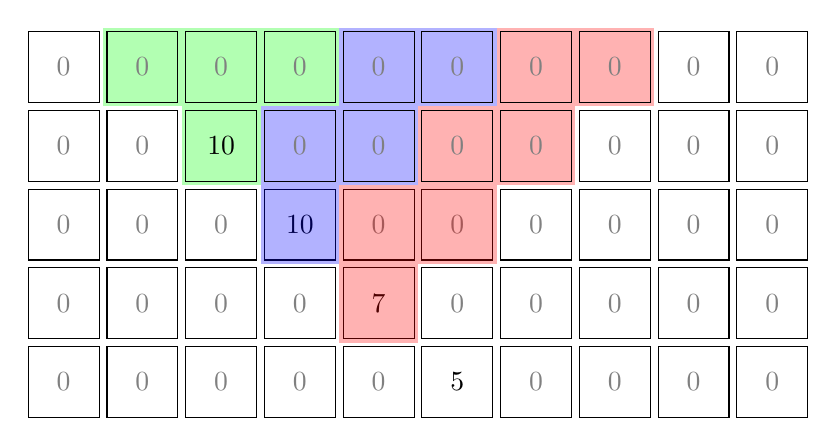
\begin{tikzpicture}[scale=1, node distance= 1cm]
\tikzstyle{block} = [rectangle, minimum width=0.9cm, minimum height=0.9cm, draw=black,align=flush left]
\tikzstyle{filledBlock} = [rectangle, minimum width=1cm, minimum height=1cm,fill opacity=0.3,,behind path]
\node (B0_0) at (0,0) [block] {\color{gray}$0$};
\node (B1_0) at (1,0) [block] {\color{gray}$0$};
\node[fill=green] (C1_4) at (1,4) [filledBlock] {};
\node (B2_0) at (2,0) [block] {\color{gray}$0$};
\node[fill=green] (C2_4) at (2,4) [filledBlock] {};
\node (B3_0) at (3,0) [block] {\color{gray}$0$};
\node[fill=green] (C3_4) at (3,4) [filledBlock] {};
\node (B4_0) at (4,0) [block] {\color{gray}$0$};
\node[fill=blue] (C4_4) at (4,4) [filledBlock] {};
\node (B5_0) at (5,0) [block] {\color{black}$5$};
\node[fill=blue] (C5_4) at (5,4) [filledBlock] {};
\node (B6_0) at (6,0) [block] {\color{gray}$0$};
\node[fill=red] (C6_4) at (6,4) [filledBlock] {};
\node (B7_0) at (7,0) [block] {\color{gray}$0$};
\node[fill=red] (C7_4) at (7,4) [filledBlock] {};
\node (B8_0) at (8,0) [block] {\color{gray}$0$};
\node (B9_0) at (9,0) [block] {\color{gray}$0$};
\node (B0_1) at (0,1) [block] {\color{gray}$0$};
\node (B1_1) at (1,1) [block] {\color{gray}$0$};
\node (B2_1) at (2,1) [block] {\color{gray}$0$};
\node[fill=green] (C2_3) at (2,3) [filledBlock] {};
\node (B3_1) at (3,1) [block] {\color{gray}$0$};
\node[fill=blue] (C3_3) at (3,3) [filledBlock] {};
\node (B4_1) at (4,1) [block] {\color{black}$7$};
\node[fill=blue] (C4_3) at (4,3) [filledBlock] {};
\node (B5_1) at (5,1) [block] {\color{gray}$0$};
\node[fill=red] (C5_3) at (5,3) [filledBlock] {};
\node (B6_1) at (6,1) [block] {\color{gray}$0$};
\node[fill=red] (C6_3) at (6,3) [filledBlock] {};
\node (B7_1) at (7,1) [block] {\color{gray}$0$};
\node (B8_1) at (8,1) [block] {\color{gray}$0$};
\node (B9_1) at (9,1) [block] {\color{gray}$0$};
\node (B0_2) at (0,2) [block] {\color{gray}$0$};
\node (B1_2) at (1,2) [block] {\color{gray}$0$};
\node (B2_2) at (2,2) [block] {\color{gray}$0$};
\node (B3_2) at (3,2) [block] {\color{black}$10$};
\node[fill=blue] (C3_2) at (3,2) [filledBlock] {};
\node (B4_2) at (4,2) [block] {\color{gray}$0$};
\node[fill=red] (C4_2) at (4,2) [filledBlock] {};
\node (B5_2) at (5,2) [block] {\color{gray}$0$};
\node[fill=red] (C5_2) at (5,2) [filledBlock] {};
\node (B6_2) at (6,2) [block] {\color{gray}$0$};
\node (B7_2) at (7,2) [block] {\color{gray}$0$};
\node (B8_2) at (8,2) [block] {\color{gray}$0$};
\node (B9_2) at (9,2) [block] {\color{gray}$0$};
\node (B0_3) at (0,3) [block] {\color{gray}$0$};
\node (B1_3) at (1,3) [block] {\color{gray}$0$};
\node (B2_3) at (2,3) [block] {\color{black}$10$};
\node (B3_3) at (3,3) [block] {\color{gray}$0$};
\node (B4_3) at (4,3) [block] {\color{gray}$0$};
\node[fill=red] (C4_1) at (4,1) [filledBlock] {};
\node (B5_3) at (5,3) [block] {\color{gray}$0$};
\node (B6_3) at (6,3) [block] {\color{gray}$0$};
\node (B7_3) at (7,3) [block] {\color{gray}$0$};
\node (B8_3) at (8,3) [block] {\color{gray}$0$};
\node (B9_3) at (9,3) [block] {\color{gray}$0$};
\node (B0_4) at (0,4) [block] {\color{gray}$0$};
\node (B1_4) at (1,4) [block] {\color{gray}$0$};
\node (B2_4) at (2,4) [block] {\color{gray}$0$};
\node (B3_4) at (3,4) [block] {\color{gray}$0$};
\node (B4_4) at (4,4) [block] {\color{gray}$0$};
\node (B5_4) at (5,4) [block] {\color{gray}$0$};
\node (B6_4) at (6,4) [block] {\color{gray}$0$};
\node (B7_4) at (7,4) [block] {\color{gray}$0$};
\node (B8_4) at (8,4) [block] {\color{gray}$0$};
\node (B9_4) at (9,4) [block] {\color{gray}$0$};
\end{tikzpicture}

%  \caption{caption}
%  \label{fig:design_guidelines}
%\end{figure}
\section{Precedencias Ordenadas}
El modelo de precedencias ordenadas es un modelo donde consideramos la mina como una serie de $n$ incrementos, apilados uno encima del otro. Sin perder generalidad, asumimos que los incrementos están ordenados de manera descendente, es decir, el incremento $1$ es el de mas arriba y debe ser el primero en extraerse, mientras que para el incremento $i > 1$, los incrementos $1,\dotsc,i-1$ debieron haber sido extraídos antes.  

\subsection{Problema de planificación}
Para modelar el problema primero decimos que una mina, una instancia, cuenta con los siguientes conjuntos:
\begin{itemize}
    \item[$\mI$] : Conjunto de incrementos
    \item[$\mB$] : Conjunto de bloques
    \item[$\mB_i$] : Conjunto de bloques en el incremento $i$
    \item[$\mT$] : Conjunto de periodos 
\end{itemize}
Además de los siguientes parámetros:
\begin{itemize}
    \item[$Q_0$] : Toneladas originales de la mina.
    \item[$g_b$] : Grado del bloque $b\in \mB$
    \item[$q_b$] : Toneladas de material en el bloque $b\in\mB$
    \item[$q_i$] : Toneladas de material en el incremento $i\in\mI$
    \item[$\pi_{m.t}$] : Costo de minar una tonelada de material en el periodo $t\in\mT$.
    \item[$\pi_{c,t}$] : Costo de concentrado de una tonelada de mineral en el periodo $t\in\mT$
    \item[$\pi_{r,t}$] : Precio de mercado de una onza de material refinado en el periodo $t\in\mT$
    \item[$\pi_{s,t}$] : Costo de vender una onza de material refinado en el periodo $t\in\mT$
    \item[$\delta$] : Tasa de descuento temporal
    \item[$y$] : Proporción del material recuperado al enviarlo al procesador y refinería.
\end{itemize}

El grado del bloque $g_b$ se entiende como la proporción de material con valor hay dentro del bloque $b\in\mB$.\\

Ya establecida la instancia del problema, definimos las variables de decisión:

\begin{itemize}
    \item[$Q_m$] : Toneladas de material extraído. 
    \item[$Q_c$] : Toneladas de material enviadas al concentrador
    \item[$Q_r$] : Onzas de material refinado obtenido
    \item[$x_i$] : Proporción extraída del incremento $i\in\mI$
    \item[$z_b$] : Proporción del bloque $b\in\mB$ enviada al concentrador en el tiempo $t\in \mT$
    \item[$\mu_i$] : Variable de precedencia binaria, indica si se extrajo el incremento $i\in\mI$
\end{itemize}

Teniendo ya las variables y parámetros del problema, podemos comenzar a definir las funciones del mismo.\\
Comenzamos definiendo $U_i(Q)$, que representa las toneladas restantes en el incremento $i$, luego de extraer $Q$ toneladas:
\begin{align*}
U_i(Q) = \Big(\min\big\{q_i,\sum\limits_{j=1}^{i} q_j-Q\big\}\Big)^+
\end{align*}
$q_i$ son las toneladas que tiene el incremento $i$.\\
Luego, definimos la siguiente función $u(Q,w,t)$ como un problema de maximización:

\[
\begin{array}{lllll}
u(Q,w,t) &  \multicolumn{4}{l}{ = \; \max \; (\pi_{r,t} - \pi_{s,t} ) Q_{r}  - \pi_{c,t} Q_{c} - \pi_{m,t} Q_{m} } \\
\text{s.a.} & & & & \\
& 0   & \leq \; z_{b} \leq x_{i} & \forall i \in 1, \ldots, n, \; p \in \mB_i, & (1)\\
& Q_{m} & = \; \sum\limits_{i = 1}^n q_i x_i = w & & (2)\\
& Q_{c} & = \; \sum\limits_{i = 1}^n \sum\limits_{b \in \mB_i} q_{b} z_{b} & & (3)\\
& Q_{r} & = \; y \sum\limits_{i = 1}^n \sum\limits_{p \in \mB_i} q_{b} g_{b} z_{b} &  & (4)\\
& Q_{m} & \leq \; M_t, & & (5)\\
& Q_{c} & \leq \; C_t, & & (6)\\
& Q_{r} & \leq \; R_t, & & (7) \\
& q_i x_{i} & \leq \; \mu_i U_i(Q_0-Q) , & \forall i \in 1, \ldots, n. & (8) \\
& q_i x_{i} & \geq \; \mu_{i+1} U_i(Q_0-Q) , & \forall i \in 1, \ldots, n. & (9) \\
& \mu_{i} & \in \; \{0,1\} & \forall i \in 1, \ldots, n.  & (10) \\
&      x_{i} & \in \; [0,1] & \forall i \in 1, \ldots, n.  & (11) \\
\end{array}
\]
\\
La función $u(Q,w,t)$ se interpreta como el máximo valor posible que se puede obtener extrayendo $w$ toneladas de material en el tiempo $t$, quedando $Q$ toneladas en la mina.\\

Habiendo definido las funciones anteriores, podemos formular el problema de planificación con la siguiente recursión:

\[
\begin{array}{lllll}
V(Q,t) &  \multicolumn{4}{l}{ = \; \max \; u(Q,w,t) + \delta^t V(Q-w,t+1) } \\
\text{s.a.} & & & & \\
& 0  \leq w \leq M_t \\
\end{array}
\]
\\

Donde $M_t$ es la cantidad máxima que se puede minar en el periodo $t$.\\
En este modelo, la función $V(Q,t)$ representa el VAN de la mina cuando quedan $Q$ toneladas en el tiempo $t$.
%\begin{itemize}
%    \item[$\delta$] : Factor de descuento %para calcular el VAN. 
%    \item[$q_b$] : Cantidad en toneladas de% material en el bloque $b \in \mB$,
%    \item[$g_{b,m}$] : Cantidad de material $m \in M$ en el bloque $b \in \mB$,
%    \item[$\pi_{r, m}$] : Precio de mercado del material refinado  $m \in \mM$,
%    \item[$\pi_{s, m}$] : Costo de venta por onza del material refinado $m \in \mM$.
%    \item[$D_b$] :  Conjunto de destinos disponibles para $b \in \mB$,
%    \item[$D_w$] : Conjunto de destinos disponibles para el almacén $w \in \mS$,
%    \item[$c_{b,d}$] : Costo de enviar una tonelada de material desde $b \in \mB$ hasta $d \in \mD_b$,
%    \item[$c_{w,d}$] : Costo de enviar una tonelada de material desde el almacén $w \in \mS$ hasta $d \in \mD_b$,
%    \item[$y_{m,d}$] : Proporción del material $m \in \mM$ recuperado utilizando el destino $d \in \mD$.
%\end{itemize}

\subsubsection{Simplificación del problema}
La formulación del problema anterior genera dos dificultades para resolverlo. La primera, es que es un problema recursivo con respecto a $V(Q,t)$, ya que se necesita información sobre $V(Q-w,t+1)$ para su calculo. La segunda se debe a que la función $u(Q,w,t)$ es también un problema de maximización, por lo que para calcular $V(Q,t)$ es necesario resolver dos problemas de maximizacion anidados.
En esta parte nos centraremos en simplificar los problemas anidados. Para facilitar el calculo, reescribimos el problema de la siguiente manera:
\\

\textbf{(P_1)}
\begin{cases}
\[
\begin{array}{lllll}
V(Q,t)  & \multicolumn{4}{l}{ = \; \max \; (\pi_{r,t} - \pi_{s,t} ) Q_{r}  - \pi_{c,t} Q_{c} - \pi_{m,t} Q_{m} + \delta^t V(Q-Q_m,t+1)} \\
\text{s.a.} & & & & \\
& 0   & \leq \; z_{b} \leq x_{i} & \forall i \in 1, \ldots, n, \; b \in \mB_i, & (1)\\
& Q_{m} & = \; \sum\limits_{i = 1}^n q_i x_i & & (2)\\
& Q_{c} & = \; \sum\limits_{i = 1}^n \sum\limits_{b \in \mB_i} q_{b} z_{b} & & (3)\\
& Q_{r} & = \; y \sum\limits_{i = 1}^n \sum\limits_{p \in I_i} q_{b} g_{b} z_{b} &  & (4)\\
& Q_{m} & \leq \; M_t, & & (5)\\
& Q_{c} & \leq \; C_t, & & (6)\\
& Q_{r} & \leq \; R_t, & & (7) \\
& q_i x_{i} & \leq \; \mu_i U_i(Q_0 -Q) , & & (8) \\
& q_i x_{i} & \geq \; \mu_{i+1} U_i(Q_0 - Q) , & & (9) \\
& \mu_{i} & \in \; \{0,1\} & \forall i \in 1, \ldots, n.  & (10) \\
&      x_{i} & \in \; [0,1] & \forall i \in 1, \ldots, n.  & (11) \\
\end{array}
\]
\end{cases}
\\

En este cambio, se agrupan ambos problemas de maximización en uno, agregando función objetivo a maximizar en $u(Q,w,t)$ y sus restricciones. De esta manera, el problema de maximización se transforma en un problema lineal que puede ser resuelto de manera más simple.

\subsubsection{Reformulación del problema}

Ahora, buscamos reescribir el problema, de tal manera que quede en función de los bloques de la mina (denotados por $\mB$) y de los destinos que estos tengan (denotados por $\mD$).\\
Además agregaremos el conjunto de las restricciones $\mR^d$, donde $d\in\mD$.
\\

\textbf{(P_2)}
\begin{cases}
\[
\begin{array}{lllll}
V(Q, t) &  \multicolumn{4}{l}{ = \; \max \; \sum\limits_{d\in\mD} \sum\limits_{b\in\mB} p_{b, d} y_{b, d}+ \delta^t V\left(Q - \sum\limits_{i\in\mI} q_i x_i, t+1\right)}\\
\text{s.t.} & & & & \\
&     &  \sum\limits_{b\in \mB} q_{b,r} y_{b, d} \leq R^r_t & \forall d\in\mD, \forall r\in \mR^d \;\;\;\;\;\;\;\;\;\;\;& (1) \\
&     &  \sum\limits_{b\in \mB} q_b \sum\limits_{d\in \mD} y_{b, d} \leq M_t  & &(2)\\
&     & x_{i}  = \; \sum\limits_{d \in \mD} y_{b,d} & \forall i \in \mI, \forall b \in \mB_i, & (3) \\
&     & q_i x_{i}  \leq \; \mu_i U_i(Q_0 -Q) ,  & \forall i \in \mI, & (4) \\
&     & q_i x_{i}  \geq \; \mu_{i+1} U_i(Q_0 -Q) ,  & \forall i \in \mI, & (5)\\
&     & \mu_{i} \in \; \{0,1\} & \forall i \in \mI, & (6) \\
&     &  y_{b,d}\in \; [0,1] & \forall b \in \mB, d \in \mD, & (7)\\
&     &  x_{i}  \in \; [0,1] & \forall i \in \mI. &  (8)\\
\end{array}
\]
\end{cases}
\vspace{8mm}
\\
El objetivo es demostrar que \textbf{(P\textsubscript{1})} puede ser reducido a \textbf{(P\textsubscript{2})} redefiniendo variables.

Para reducir el problema, definimos más detalladamente el conjunto de destinos $\mD$. En este caso solo tomaremos $\mD =\{1,2\}$ (el problema solo tiene dos direcciones), donde $d=1$ representa el concentrador y $d=2$ el botadero.

\paragraph{Función Objetivo}

Primero, comenzaremos reformulando la función objetivo, Para esto, podemos reemplazar las variables $Q_r,Q_c,Q_m$ de la siguiente forma

\begin{align*}
     (\pi_{r,t} - \pi_{s,t} ) Q_{r}  - \pi_{c,t} Q_{c} - \pi_{m,t} Q_{m} = & \pi_{r,s,t}  \,y \sum\limits_{i = 1}^n \sum\limits_{b \in \mB_i} q_{b} g_{b} z_{b}  - \pi_{c,t} \sum\limits_{i = 1}^n \sum\limits_{b \in \mB_i} q_{b} z_{b} - \pi_{m,t} \sum\limits_{i = 1}^n q_i x_i\\
     = & \sum\limits_{i=1}^n \sum\limits_{b \in \mB_i}\{ z_b q_b(\pi_{r,s,t} y g_b+\pi_{c,t}) \} - \pi_{m,t} q_i x_i
\end{align*}
Donde $\pi_{r,s,t} = \pi_{r,t}-\pi_{s,t}$.\\
Definimos los siguientes cambios:
\begin{align*}
\begin{cases}
y_{b,1} & =z_b\\
y_{b,2} & =\sum \limits_{i=1}^n(x_i -z_b)\Ind_{b\in \mB_i} \\
\sum \limits_{i=1}^n q_i x_i & =\sum\limits_{b\in\mB}\sum \limits_{d \in \mD} q_b y_{b,d} 
\end{cases}
\end{align*}

La variable $y_{b,d}$ representa la cantidad del bloque $b\in\mB$ que se lleva al destino $d\in\mD$\\
Notemos que $y_{b,d}\in [0,1]$, dado que $0\leq z_p \leq x_i \;\; \forall i \in 1,\ldots,n, \; p \in I_i$ y además $x_i \in [0,1]$.\\

Además cumple la igualdad $(3)$ de \textbf{(P\textsubscript{2})}:
$$
 \sum\limits_{d \in \mD} y_{b,d}  
=  y_{b,1} + y_{b,2} 
= z_b + \sum \limits_{i=1}^n(x_i -z_b)\Ind_{b\in \mB_i} 
= x_i \;\;\; \forall i \in \mI, \forall b \in \mB_i,\\
$$

Con esto podemos simplificar el problema :
\begin{align*}
    \sum\limits_{i=1}^n \sum\limits_{b \in \mB_i}\{ z_b q_b(\pi_{r,s,t} y g_b+\pi_{c,t}) \} - \pi_{m,t} q_i x_i = & \sum\limits_{b \in \mB}  y_{b,1} q_b(\pi_{r,s,t} y g_b+\pi_{c,t})  - \pi_{m,t} q_b (y_{b,1}+y_{b,2})\\
= &\sum\limits_{b \in \mB}  y_{b,1} (q_b(\pi_{r,s,t} y g_b+\pi_{c,t}-\pi_{m,t}))  - \pi_{m,t} q_b y_{b,2}\\
= & \sum \limits_{b \in \mB} p_{b,1}y_{b,1} +p_{b,2}y_{b,2} = \sum \limits_{b \in \mB} \sum \limits_{d \in \mD} p_{b,d}y_{b,d}
\end{align*}

Aquí, utilizamos $p_{b,1} = q_b(\pi_{r,s,t} y g_b+\pi_{c,t}-\pi_{m,t})$, $p_{b,2} = - \pi_{m,t} q_b $.\\

\paragraph{Restricciones $\mR^d$}
Luego para redefinir las restricciones, usamos:
\begin{align*}
\text{Para $d=1$, tenemos :}
\begin{cases}
\mR^1= \{1,2\}\\
q_{b,1}= q_b\\
q_{b,2}=q_b y g_b\\
R_t^1= C_t\\
R_t^2= R_t\\
\end{cases}
\end{align*}

Dado que para $d=2$ (el botadero) no hay restricciones, tenemos $\mR^2 = \emptyset$

Usando esto tenemos:
\begin{align*}
\bigcdot &  \sum\limits_{i=1}^n  \sum\limits_{b \in \mB_i}\ q_b z_b\ \leq C_t \\
\Rightarrow & \sum\limits_{b \in \mB} \ q_{b,1} y_{b,1} \leq R_t^1 \\
\bigcdot & \sum\limits_{i=1}^n  \sum\limits_{b \in \mB_i}\  y q_b z_b g_b\ \leq R_t \\
\Rightarrow & \sum\limits_{b \in \mB} \ q_{b,2} y_{b,1} \leq R_t^2 \\
\end{align*}

Luego agrupamos ambos restricciones iterando sobre d y r:
\begin{align*}
&   \sum\limits_{b \in \mB} \ q_{b,r} y_{b,d} \leq R_t^r, \;\;\; \forall d\in\mD, \forall r\in \mR^d\\
\end{align*}

\paragraph{Restricciones $M_t$}
Usando el mismo cambio anterior con $\sum \limits_{i=1}^n q_i x_i & = \sum\limits_{b\in\mB}\sum \limits_{d \in \mD} q_b y_{b,d} $ obtenemos :
$$
Q_m = \sum \limits_{i=1}^n q_i x_i \leq M_t \Rightarrow \sum\limits_{b\in\mB}\sum \limits_{d \in \mD} q_b y_{b,d}\leq M_t
$$
\\
Con esto, obtenemos un modelo \textbf{(P\textsubscript{2})} indexado por los conjuntos $\mB$, $\mD$ y $\mR$
A partir de aquí, solo queda buscar resolver el problema de recursividad de $V(Q,t)$, además de implementar un algoritmo de programación dinámica.
\newpage
\subsection{Implementación}

Para implementar un algoritmo de programación dinámica se propone crear una sucesión recursiva de $(V_k)_{k=1}^n$ que resuelva el problema para cada iteración $k$. Con esto, el problema de planificación queda de la siguiente manera :

\[
\begin{array}{lllll}
V^k(Q,t) &  \multicolumn{4}{l}{ = \; \max \; u(Q,w,t) + \delta^t V^{k-1}(Q-w,t+1) } \\
\text{s.a.} & & & & \\
& 0  \leq w \leq M_t \\
\end{array}
\]

Para el paso inicial, utilizaremos $V^0(Q,t).=0, \;\; \forall Q>0, \forall t \in \mT$. 
Con esta recursión ya definida, implementamos el siguiente algoritmo : 
\begin{algorithm}
\caption{Programación dinámica}\label{alg:dp}
\KwIn{Input}
\KwOut{Output}

Definir $V^0(Q,t) = 0, \forall Q \geq 0, \forall t \in \mT$.\\ 
Definir  $k=1$.\\

\Repeat{$v_k \leq v_{k-1}$}
{
$t \leftarrow 1$,\\
$Q^k \leftarrow \sum\limits_{i=1}^n q_i,$\\
$v^k \leftarrow 0,$

\While{$Q^k > 0$ and $t \in \mT$}
{
$
\begin{array}{lll}
V^k(Q^k,t)  =  & \max & u(Q^k,q,t) + \delta^t V^{k-1}(Q^k - q, t+1) \\
            & \text{s.t.} &    \\
            & &  0 \leq q \leq \min\{Q^k, M_{t}\} \\
\end{array}
$

Extraer $\bar q$, que maximiza $V^k(Q^k,t)$.\\ 
Extraer $\bar x, \bar z$ que maximiza $u(\bar q, t)$.\\  

$x_{t}^k \leftarrow \bar x$.\\
$z^k_{t} \leftarrow \bar z$.\\
$Q^k \leftarrow Q^k - \bar q$.\\
$v^k \leftarrow v^k + \delta^t u(\bar q,t)$.\\
$t \leftarrow t+1.$\\

}
Definir $V^k(Q,t)$ Para todos los valores $Q \geq 0$ y $t \in \mT$.\\
$k \leftarrow k+1$\\
}
$x^* \leftarrow x^{k-1}$.
\end{algorithm}

Este algoritmo, presenta el problema de calcular la función $V^{k-1}(Q,t)$ para cada $(Q,t)$. Para esto definimos el valor anterior de la mina $V^{k-1}_0$ como:

$$ V^{k-1}_0 = \sum_{t \in \mT} \delta^{t-1} u(q^{k-1}_{t},t)$$

Donde $q^{k-1}_{t}$ es las toneladas extraídas de la mina en la iteración $k-1$ para el periodo $t$. Con esto generamos una serie de valores $V^{k-1}_t,Q^{k-1}_t$ de la forma

$$  V^{k-1}_t =  V^{k-1}_0 - \sum_{j \in \mT, j <= t} \delta^{j-1} u(q^{k-1}_{j},j) $$

$$Q^{k-1}_0 = Q_0, \quad  Q^{k-1}_t =  Q^{k-1}_0 - \sum_{j \in \mT, j <= t} q^{k-1}_{j}$$

Así, estimamos la función $V^{k-1}(Q,t)$ como una función lineal por partes en función de la variable $Q$, dada por los puntos $\{V^{k-1}_t,Q^{k-1}_t\}_{t \in \mT}$. Además se consideran los puntos de borde $(V^{k-1}_0,Q_0)$; en un principio tengo todo el valor de la mina, y $(0,0)$; si no quedan toneladas entonces la mina no tiene valor. \\

Para implementar este algoritmo se utilizó Python 3.7.3, para la parte de optimización y la función lineal por partes se utilizó Gurobi 9.5.0. 


\subsection{Problema de extracción}

Debido a la formulación de $V^k$, dependiendo de los bloques e incrementos, el algoritmo a veces decide no extraer nada de la mina, debido a que estima mas beneficioso no hacerlo. Para obligar la extracción de mineral en todas las iteraciones, se agregan las siguientes variables y restricciones :

\begin{align*}
\begin{cases}
\frac{R_t^r-\sum\limits_{b \in \mB} q_{b,r}y_{b,d}}{R_t^r} &\leq \mu_r \\
\frac{M_t- \sum \limits_{b\in \mB}\sum\limits_{ d \in \mD} q_b y_{b,d}}{M_t} &\leq  \mu_M\\
\mu_M + \sum\limits_{r\in \mR} \mu_r &\leq  \abs{\mR}\\
\mu_M, \, \mu_r \in \{0,1\} &\forall r \in \mR
\end{cases}
\end{align*}

Con estas restricciones, se obliga al algoritmo a extraer al menos $\mR_t^r$ o $M_t$.

Claramente en esta formulación se puede obtener utilidades negativas. Para evitar este problema se aplica un método de post-optimización, extrayendo los incrementos finales de la solución, es decir, si se extraen los incrementos $1,\dotsc,k$, entonces se descartan, en caso de existir, los incrementos $j,\dotsc,k$, con $j\leq k$, tales que sus utilidades son negativas.

\subsection{Resultados}

\begin{table}[H]
\centering
\begin{tabular}{|l|cccc|}
\hline
                 & \textbf{OMP IP} & \textbf{Modelo Libre} & \textbf{Modelo Restringido} & \textbf{OMP LP} \\ \hline
\textbf{Chaiten} & 233.986                   & 129.100(k = 2)               & 237.179(k = 2)                     & 294.391                    \\ \hline
\textbf{KD}      & 310.028                   & 241.518(k = 2)               & 306.483(k = 6)                    & 333.120                    \\ \hline
\textbf{Marvin}  & 797.463                   & 470.450(k = 2)               & 796.491(k = 3)                     & 905.751                    \\ \hline
\textbf{Palomo}  & 162.704                   & 858.866(k = 4)               & 603.336(k = 3)                    & 6073.318                   \\ \hline
\end{tabular}
\caption{Valor estimado de la mina (Restringida a los incrementos utilizados en la solución OMP IP)[\$1.000.000]. La cantidad de iteraciones realizadas por el algoritmo viene dado por el número k.}
\end{table}

\begin{table}[H]
\centering
\begin{tabular}{|l|cccc|}
\hline
                 &\textbf{OMP IP} & \textbf{Modelo Libre} & \textbf{Modelo Restringido} & \textbf{OMP LP} \\ \hline
\textbf{Chaiten} & 233.986                   & 129.100(k = 2)               & 234.766(k = 2)                     & 294.391                    \\ \hline
\textbf{KD}      & 310.028                   & 349.155(k = 4)               & 361.183(k = 6)                     & 333.120                    \\ \hline
\textbf{Marvin}  & 797.463                   & 470.450(k = 2)               & 794.728(k = 3)                     & 905.751                    \\ \hline
\textbf{Palomo}  & 162.704                   & 858.866(k = 4)               & 603.336(k = 2)                   & 6073.318                   \\ \hline
\end{tabular}
\caption{Valor estimado de la mina [\$1.000.000]. La cantidad de iteraciones realizadas por el algoritmo viene dado por el número k.}
\end{table}

\begin{table}[H]
\centering
\begin{tabular}{|l|cc|cc|}
\hline
\multirow{2}{*}{} & \multicolumn{2}{c|}{\textbf{Incrementos Filtrados}}  & \multicolumn{2}{c|}{\textbf{Incrementos no Filtrados}}   \\ \cline{2-5} 
                  & \textbf{Modelo Libre} & \textbf{Restringido} & \textbf{Modelo Libre} & \textbf{Restringido} \\ \hline
\textbf{Chaiten}  & 13.1                  & 57.5                        & 14.2                  & 86.5                            \\ \hline
\textbf{KD}       & 0.3                   & 0.7                         & 2.9                   & 1.3                             \\ \hline
\textbf{Marvin}   & 0.8                   & 1.4                         & 2.4                   & 4.7                             \\ \hline
\textbf{Palomo}   & 11.2                  & 4.9                         & 34.5                & 33.5                            \\ \hline
\end{tabular}
\caption{Tiempo que tomó el algoritmo en encontrar una solución para cada problema [Minutos]}
\end{table}

\begin{table}[H]
\centering
\begin{tabular}{|l|cccc|}
\hline
\multirow{2}{*}{} & \multicolumn{1}{l|}{\multirow{2}{*}{\textbf{OMP IP}}} & \multicolumn{2}{c|}{\textbf{Modelo Libre}}                                     & \multicolumn{1}{l|}{\multirow{2}{*}{\textbf{OMP LP}}} \\ \cline{3-4}
                  & \multicolumn{1}{l|}{}                        & \textbf{Incrementos Filtrados} & \multicolumn{1}{c|}{\textbf{Incrementos no Filtrados}} & \multicolumn{1}{l|}{}                        \\ \hline
\textbf{Chaiten}  & 233.986                                      & 129.417(k = 2)        & 129.417(k = 2)                                & 294.391                                      \\ \hline
\textbf{KD}       & 310.028                                      & 241.517(k = 2)        & 331.469(k = 3)                                & 333.120                                      \\ \hline
\textbf{Marvin}   & 797.463                                      & 498.472(k = 2)        & 498.472(k = 2)                                & 905.751                                      \\ \hline
\textbf{Palomo}   & 162.704                                      &                       &                                               & 6073.318                                     \\ \hline
\end{tabular}
\caption{Valor estimado de la mina [\$1.000.000], restringiendo la variable a x a los valores 0 o 1.}
\end{table}

\begin{table}[H]
\centering
\begin{tabular}{|l|cc|}
\hline
\multicolumn{1}{|l|}{\multirow{2}{*}{}} & \multicolumn{2}{c|}{\textbf{Modelo Libre}}                         \\ \cline{2-3} 
\multicolumn{1}{|l|}{}                  & \textbf{Incrementos Filtrados} & \textbf{Incrementos no Filtrados} \\ \hline
\textbf{Chaiten}                        & 10.9                           & 11.5                              \\ \hline
\textbf{KD}                             & 0.3                            & 0.8                               \\ \hline
\textbf{Marvin}                         & 0.7                            & 1.1                               \\ \hline
\textbf{Palomo}                         &                                &                                   \\ \hline
\end{tabular}
\caption{Tiempo que tomó el algoritmo en encontrar una solución para cada problema [Minutos]}
\end{table}

\begin{table}[H]
\centering
\begin{tabular}{|l|cccc|}
\hline
                 & \multicolumn{1}{l}{\textbf{OMP IP}} & \textbf{Modelo Libre} & \textbf{Modelo Restringido} & \multicolumn{1}{l}{\textbf{OMP LP}} \\ \hline
\textbf{Chaiten} & 233.986                             & 120.100(k = 3)        & 217.285(k = 3)              & 294.391                             \\ \hline
\textbf{KD}      & 310.028                             & 361.379(k = 3)        & 361.379(k = 3)              & 333.120                             \\ \hline
\textbf{Marvin}  & 797.463                             & 470.449(k = 3)        & 794.943(k = 3)              & 905.751                             \\ \hline
\textbf{Palomo}  & 162.704                             &                       &                             & 6073.318                            \\ \hline
\end{tabular}
\caption{Valor estimado de la mina [\$1.000.000], utilizando la solución IP de OMP para estimar la función $V^0(Q,t)$.}
\end{table}

\begin{table}[H]
\centering
\begin{tabular}{|l|cc|}
\cline{1-3}
                 & \textbf{Modelo Libre} & \textbf{Modelo Restringido} \\ \hline
\textbf{Chaiten} & 18.1                  &  162.5                       \\ \hline
\textbf{KD}      & 1.2                   & 0.7                         \\ \hline
\textbf{Marvin}  & 1.6                   & 17.5                        \\ \hline
\textbf{Palomo}  &                       &                             \\ \hline
\end{tabular}
\caption{Tiempo que tomó el algoritmo en encontrar una solución para cada problema [Minutos]}
\end{table}

\subsubsection{ Discusión de resultados}

En la primera tabla se observan los resultados con el proceso que considera solo los incrementos que fueron utilizados en la solución previa. Para este caso, obtenemos valores muy cercanos a los observados en la solución previa para todas las instancias, con la excepción de Palomo. Se realizan solo dos iteraciones para todas las instancias menos Palomo, esto no permite analizar la convergencia. Sin embargo, al alterar la condición de termino permitiendo un mayor número de iteraciones, no se encuentran mejores soluciones y converge a una función periódica que oscila entre dos valores, esto sugiere que el modelo no es capaz de salir de ciertas estimaciones de la función V, esto se podría solucionar generando alguna cantidad de ruido en la función V para que logre salir de estas oscilaciones.

En la segunda tabla, donde consideramos todos los incrementos. Nuestro modelo supera a la relajación lineal previa para KD, esto es causado porque los incrementos no considerados en la solución previa son utilizados por nuestra solución y estos permiten conseguir un mayor valor objetivo. En el caso de Chaitén y Marvin, nuestra solución es ligeramente menor a la obtenida en la Tabla 1, esto puede ser causado por que el modelo no es capaz de explorar ciertas soluciones considerando todos los incrementos que si logra explorar al simplificar el modelo.

\section{Precedencias generales}
En el caso anterior, consideramos que la mina estaba ordenada solo por los incrementos $i$ de manera vertical. Para el siguiente modelo, consideraremos que la mina esta ordenada por 2 parámetros $(i,p)$, donde $i$ son los Bancos horizontales y $p$ las Fases verticales de la mina. Este par ordenado $(i,p)$ es el incremento. Debido a que la mina ahora está indexada por un par ordenado, se pierde el orden total de la mina, por lo que es necesario crear una nueva regla de precedencia para poder extraer los incrementos.\\

Estas reglas, para un incremento $(i,p)$ son las siguientes (asumimos que tanto bancos como fases van en orden ascendente):
\begin{itemize}
    \item[\textbf{(a)}] El incremento $(0,0)$ no tiene precedencias (es el incremento que se extrae primero)
    \item[\textbf{(b)}]El incremento $(i,p)$ tiene como precedencias : $\begin{cases}
    \bigcdot \;(i-1,p) \textbf{ si } $i>0$.\\
    \bigcdot \; (i,p-1)  \textbf{ si } $p>0$.
    \end{cases}$
\end{itemize}

Con esto, el bloque $(i,p)$ puede tener más de una precedencia, dependiendo de donde se encuentre.

\subsection{Problema de planificación}

Teniendo ya las reglas de precedencias definidas, podemos comenzar a redefinir el problema de planificación. Para esto, cambiamos algunas variables, comenzamos denotando los siguientes conjuntos y parámetros:

\begin{itemize}
    \item[$\mI$] : Conjunto de bancos de la mina
    \item[$\mP$] : Conjunto de fases de la mina
    \item[$\mB$] : Conjunto de bloques de la mina
    \item[$\mB_{i,p}$] : Conjunto de bloques en el incremento $(i,p)$
    \item[$q_{b,r}$] : Cantidad de material en toneladas del bloque $b$ enviado a la restricción $r$
    \item[$q_{i,p}$] : Cantidad de material en el incremento $(i,p)$ 
\end{itemize}

Las nuevas variables del nuevo problema son las siguientes :

\begin{itemize}
    \item[$x_{i,p}$] : Proporción extraída del incremento $(i,p)$
    \item[$\mu_{i.p}$] : Variable de precedencia binaria, indica si se extrajo el incremento $(i,p)$
\end{itemize}

La función $U_{i,p}(Q)$ representa la cantidad de material en toneladas que queda en el incremento $(i.p)$ luego de extraer $Q$ toneladas de la mina.

Con los parámetros y variables ya definidas y manteniendo la notación del caso de precedencias ordenadas, podemos definir el problema de planificación :
\\
    
\textbf{(P_2^{*})}
\begin{cases}
\[
\begin{array}{lllll}
V(Q, t) &  \multicolumn{4}{l}{ = \; \max \; \sum\limits_{d\in\mD} \sum\limits_{b\in\mB} p_{b, d} y_{b, d}+ \delta^t V\left(Q - \sum\limits_{i\in\mI} \sum\limits_{p \in \mP}q_{i,p} x_{i,p}, t+1\right)}\\
\text{s.t.} & & & & \\
&     &  \sum\limits_{b\in \mB} q_{b,r} y_{b, d} \leq R^r_t & \forall d\in\mD, \forall r\in \mR^d \;\;\;\;\;\;\;\;\;\;\;& (1) \\
&     &  \sum\limits_{b\in \mB} q_b \sum\limits_{d\in \mD} y_{b, d} \leq M_t  & & (2)\\
&     & x_{i,p}  = \; \sum\limits_{d \in \mD} y_{b,d} & \forall i \in \mI, \forall p \in \mP, \forall b \in \mB_{i,p} & (3) \\
&     & q_{i.p} x_{i,p}  \leq \; \mu_{i,p} U_{i,p}(Q_0-Q) ,  & \forall i \in \mI,\;\forall p \in \mP & (4) \\
&     & q_{i,p} x_{i,p}  \geq \; \mu_{i,p+1} U_{i,p}(Q_0-Q) ,  & \forall i \in \mI,\; \forall p \in \mP & (5)\\
&     & q_{i,p} x_{i,p} \geq \mu_{i+1,p} U_{i,p}(Q_0-Q) &\forall i \in \mI,\; \forall p \in \mP  & (6)\\
&     & \mu_{i,p} \in \; \{0,1\} & \forall i \in \mI,\; \forall p \in \mP & (7) \\
&     &  y_{b,d}\in \; [0,1] & \forall b \in \mB,\; \forall d \in \mD & (8)\\
&     &  x_{i,p}  \in \; [0,1] & \forall i \in \mI, \; \forall p \in \mP &  (9)\\
\end{array}
\]
\end{cases}
\\
\\

Con el problema ya definido, se implementa un algoritmo de programación dinámica similar al caso con precedencias ordenadas.
\subsection{Resultados}

\begin{table}[H]
\centering
\begin{tabular}{|l|cccc|}
\hline
                 & \textbf{OMP IP} & \textbf{Modelo Libre} & \textbf{Modelo Restringido} & \textbf{OMP LP} \\ \hline
\textbf{Chaiten} &     233.986030               & 122.295742             & 219.468382                      &          294.390744           \\ \hline
\textbf{KD}      & 310.027537                 & 242.06336              & 292.400374                     & 333.119759
                    \\ \hline
\textbf{Marvin}  & 797.462630
                  & 473.227693               & 790.100821                     &  905.751378
                \\ \hline
\textbf{Palomo}  & 162.703768
                  &              &  -1283.721209                     &  6073.318288
                  \\ \hline
\end{tabular}
\caption{Valor estimado de la mina [\$1.000.000]. La cantidad de iteraciones realizadas por el algoritmo viene dado por el número k.}
\end{table}

\begin{table}[H]
\centering
\begin{tabular}{|l|cc|}
\hline
                 & \textbf{Modelo Libre} & \textbf{Modelo Restringido} \\ \hline
\textbf{Chaiten} & 170.96                & 728.84                      \\ \hline
\textbf{KD}      & 1.24                  & 9.88                        \\ \hline
\textbf{Marvin}  & 6.47                  & 20.90                       \\ \hline
\textbf{Palomo}  &                       & 107.28                      \\ \hline
\end{tabular}
\caption{Tiempo que tomó el algoritmo en encontrar una solución para cada problema [Minutos]}
\end{table}

\section{Mejoras}
\subsection{Condición de Cauchy}
Para mejorar la condición de término del algoritmo, se implementa una condición de Cauchy sobre la sucesión de valores obtenidos por el mismo.\\
La condición es la siguiente :
$$
\forall \varepsilon>0, \exists N \in \mathbb{N}, \forall n,m\geq N, \abs{V_n-V_m}\leq \varepsilon.
$$
En este caso, $(V_k)_{k\in\mathbb{N}}$ es la sucesión de valores obtenidos de la función objetivo. El epsilon utilizado es el $1\%$ del último $V_k$ obtenido, mientras que el $N$ utilizado es la posición $\lfloor \frac{k}{2} \rfloor$.\\
En caso de que el algoritmo no termine con esta condición de parada, se fija un $k_{maximo}$ y extrae el máximo valor de todas las iteraciones.\\

Para implementar la condición, asignamos $k_{maximo}=10$. Si el algoritmo converge en \textbf{k*} iteraciones, este terminará y entregará el valor final y la iteración \textbf{k*}
Si no converge, $\mathbf{k^*}$ representará la iteración en la cual se logró el máximo.

\subsubsection{Resultados Precedencias Ordenadas}

\begin{table}[H]
\centering
\begin{tabular}{|l|ll|lll|}
\hline
                 & \multicolumn{2}{c|}{\textbf{Modelo Restringido}} & \multicolumn{3}{c|}{\textbf{Iteraciones Cauchy}}                   \\ \cline{2-6} 
                 & \textbf{Cóncavo}         & \textbf{Cauchy}       & \textbf{Iter. Totales} & \textbf{k*} & \textbf{Convergencia} \\ \hline
\textbf{Chaiten} & 234.766 (k = 2)          & 234.765               & 10                           & 2           & \textbf{No Converge}           \\ \hline
\textbf{KD}      & 361.183 (k = 6)          & 361.182               & 5                            & 5           & \textbf{Converge}              \\ \hline
\textbf{Marvin}  & 677.164 (k = 3)          & 678.984               & 10                           & 2           & \textbf{No Converge}           \\ \hline
\textbf{Palomo}  & -2252.211 (k = 2)        &                       &                              &             &                       \\ \hline
\end{tabular}
\caption{Valor estimado de la mina [\$1.000.000]. La cantidad de iteraciones realizadas por el algoritmo cóncavo viene dado por el número k.}
\end{table}

\begin{table}[H]
\centering
\begin{tabular}{|l|ccc|}
\hline
                 & \textbf{Modelo Restringido} & \textbf{Modelo Restringido (Cauchy)} & \textbf{Convergencia}  \\ \hline
\textbf{Chaiten} & 86.5                 & 1206              & \textbf{No Converge}                              \\ \hline
\textbf{KD}      & 1.3                   & 8.95               & \textbf{Converge}                                     \\ \hline
\textbf{Marvin}  & 4.7                 & 52.60              & \textbf{No Converge}                                    \\ \hline
\textbf{Palomo}  & 33.5                 &                &                                    \\ \hline
\end{tabular}
\caption{Tiempo que tomó el algoritmo en encontrar una solución para cada problema
[Minutos]}
\end{table}


\begin{table}[H]
\centering
\begin{tabular}{|l|ll|lll|}
\hline
                 & \multicolumn{2}{c|}{\textbf{Modelo Libre}} & \multicolumn{3}{c|}{\textbf{Iteraciones Cauchy}}                   \\ \cline{2-6} 
                 & \textbf{Cóncavo}         & \textbf{Cauchy}       & \textbf{Iter. Totales} & \textbf{k*} & \textbf{Convergencia} \\ \hline
\textbf{Chaiten} & 129.100 (k = 2)                  & 129.099              & 10                           & 1           & \textbf{No Converge}           \\ \hline
\textbf{KD}      & 349.155 (k = 4)                   & 349.154             & 10                            & 3           & \textbf{No Converge}              \\ \hline
\textbf{Marvin}  & 470.450 (k = 2)                   &  470.450                & 10                         & 2           & \textbf{No Converge}           \\ \hline
\textbf{Palomo}  & 858.866 (k = 4)                 & 858.866                  & 10                             & 3            & \textbf{No converge}         \\ \hline
\end{tabular}
\caption{Valor estimado de la mina [\$1.000.000]. La cantidad de iteraciones realizadas por el algoritmo viene dado por el número k.}
\end{table}

\begin{table}[H]
\centering
\begin{tabular}{|l|ccc|}
\hline
                 & \textbf{Modelo Libre} & \textbf{Modelo Libre (Cauchy)} & \textbf{Convergencia}  \\ \hline
\textbf{Chaiten} & 14.2                &  83.59            & \textbf{No Converge}                              \\ \hline
\textbf{KD}      & 2.9                   &  37.77              & \textbf{No Converge}                                     \\ \hline
\textbf{Marvin}  & 2.4                 & 41.18              & \textbf{No Converge}                                    \\ \hline
\textbf{Palomo}  & 34.5                 &    90.67           &      \textbf{No Converge}                              \\ \hline
\end{tabular}
\caption{Tiempo que tomó el algoritmo en encontrar una solución para cada problema
[Minutos]}
\end{table}



\subsubsection{Resultados Precedencias Generales}

\begin{table}[H]
\centering
\begin{tabular}{|l|ll|lll|}
\hline
                 & \multicolumn{2}{c|}{\textbf{Modelo Libre}} & \multicolumn{3}{c|}{\textbf{Iteraciones Cauchy}}                   \\ \cline{2-6} 
                 & \textbf{Cóncavo}         & \textbf{Cauchy}       & \textbf{Iter. Totales} & \textbf{k*} & \textbf{Convergencia} \\ \hline
\textbf{Chaiten} &     122.295             & 122.295          & 10                           & 1           & \textbf{No Converge}           \\ \hline
\textbf{KD}      &     242.063             & 291.372            &       6                    & 6          & \textbf{Converge}              \\ \hline
\textbf{Marvin}  &     473.227           & 640.450              & 10                         & 4           & \textbf{No Converge}           \\ \hline
\textbf{Palomo}  &                 &                        &                              &             & \textbf{}         \\ \hline
\end{tabular}
\caption{Valor estimado de la mina [\$1.000.000]. La cantidad de iteraciones realizadas por el algoritmo viene dado por el número k.}
\end{table}

\begin{table}[H]
\centering
\begin{tabular}{|l|ccc|}
\hline
                 & \textbf{Modelo Libre} & \textbf{Modelo Libre (Cauchy)} & \textbf{Convergencia}  \\ \hline
\textbf{Chaiten} &  170.96              & 73.97            & \textbf{No Converge}                              \\ \hline
\textbf{KD}      &  1.24            & 7.43             & \textbf{Converge}                                     \\ \hline
\textbf{Marvin}  &  6.47                & 6.18             & \textbf{No Converge}                                    \\ \hline
\textbf{Palomo}  &                  &             &      \textbf{}                              \\ \hline
\end{tabular}
\caption{Tiempo que tomó el algoritmo en encontrar una solución para cada problema
[Minutos]}
\end{table}

\begin{table}[H]
\centering
\begin{tabular}{|l|ll|lll|}
\hline
                 & \multicolumn{2}{c|}{\textbf{Modelo Restringido}} & \multicolumn{3}{c|}{\textbf{Iteraciones Cauchy}}                   \\ \cline{2-6} 
                 & \textbf{Cóncavo}         & \textbf{Cauchy}       & \textbf{Iter. Totales} & \textbf{k*} & \textbf{Convergencia} \\ \hline
\textbf{Chaiten} &               &           & 10                           & 1           & \textbf{}           \\ \hline
\textbf{KD}      &     292.400        & 292.017            &      4                    & 4          & \textbf{Converge}              \\ \hline
\textbf{Marvin}  &      790.100       & 790.100             & 10                         & 5           & \textbf{No Converge}           \\ \hline
\textbf{Palomo}  &                 &                        &                              &             & \textbf{}         \\ \hline
\end{tabular}
\caption{Valor estimado de la mina [\$1.000.000]. La cantidad de iteraciones realizadas por el algoritmo viene dado por el número k.}
\end{table}

\begin{table}[H]
\centering
\begin{tabular}{|l|ccc|}
\hline
                 & \textbf{Modelo Restringido} & \textbf{Modelo Restringido (Cauchy)} & \textbf{Convergencia}  \\ \hline
\textbf{Chaiten} &               &            & \textbf{}                              \\ \hline
\textbf{KD}      &     9.88               &  4.81           & \textbf{Converge}                                     \\ \hline
\textbf{Marvin}  &  20.90                &     41.22         & \textbf{No converge}                                    \\ \hline
\textbf{Palomo}  &                  &             &      \textbf{}                              \\ \hline
\end{tabular}
\caption{Tiempo que tomó el algoritmo en encontrar una solución para cada problema
[Minutos]}

\end{table}

\subsection{Análisis de resultados}
Con los resultados del método de Cauchy, podemos notar que en general no hay muchas diferencias entre el máximo obtenido con el método de parada cóncavo y el de Cauchy. En muchos casos el máximo resulta ser similar (o el mismo valor incluso). En algunos casos, como en el modelo de precedencias generales libres, el máximo obtenido es mayor al óptimo encontrado anteriormente, esto debido a que el algoritmo continúa iterando y vuelve a encontrar otro máximo que cumple con la condición de Cauchy.\\
Sin embargo, donde se ven más diferencias es en el tiempo de ejecución del algoritmo. En general, con el método de Cauchy, el algoritmo tiende a demorar bastante más, ya que en el caso de que la sucesión no converja, el algoritmo iterará $k_{máx}$ veces, mientras que con el método cóncavo, la cantidad de iteraciones es mucho menor.\\

Con esto, podemos concluir que el método de parada cóncavo es lo suficientemente bueno para encontrar una solución óptima, si bien el método de Cauchy encuentra mejores soluciones en algunos casos, este suele demorarse mucho más que el algoritmo cóncavo, por lo que a la hora de elegir alguna condición de parada para una instancia cualquiera, lo más recomendable sea utilizar el algoritmo cóncavo, ya que probablemente obtenga una solución más rápidamente.

\section{Anexo}

\subsection{Precedencias Ordenadas}
\subsubsection{Gráficos Chaitén}

\begin{figure}[H]
  \captionsetup[subfigure]{labelformat=empty}
  \centering
  
   \textbf{Incrementos filtrados (Libre)}
  
  \begin{subfigure}[b]{0.4\textwidth}
     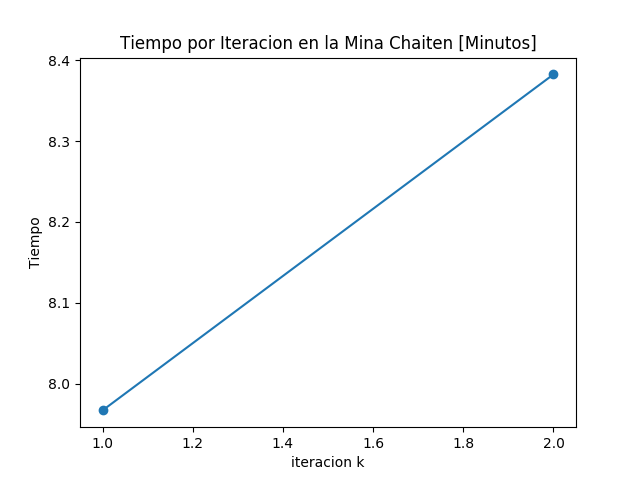
\includegraphics[width=\textwidth]{Graficos/Incrementos_filtrados/libre/chaiten_inc_times.png}
     \caption{}
     \label{asda}
  \end{subfigure}
  \begin{subfigure}[b]{0.4\textwidth}
     \includegraphics[width=\textwidth]{Graficos/Incrementos_filtrados/libre/chaiten_inc_v_k.png}
     \caption{}
     \label{fig:ex2}
  \end{subfigure}
  
  \textbf{Incrementos filtrados (Restringido)}
  
  \begin{subfigure}[b]{0.4\textwidth}
     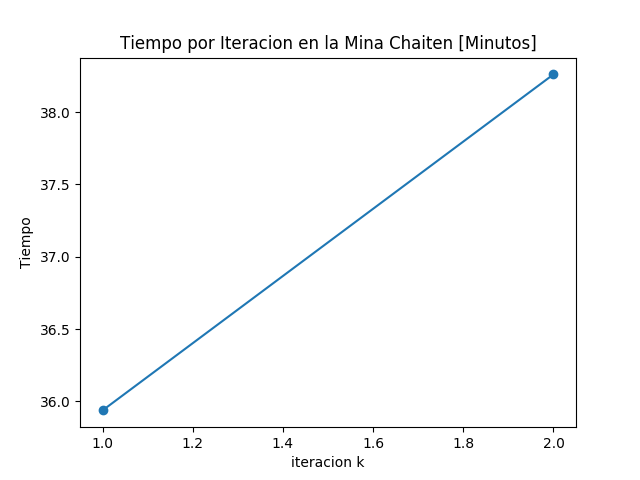
\includegraphics[width=\textwidth]{Graficos/Incrementos_filtrados/restringido/chaiten_inc_times.png}
     \caption{}
     \label{fig:ex1}
  \end{subfigure}
  \begin{subfigure}[b]{0.4\textwidth}
     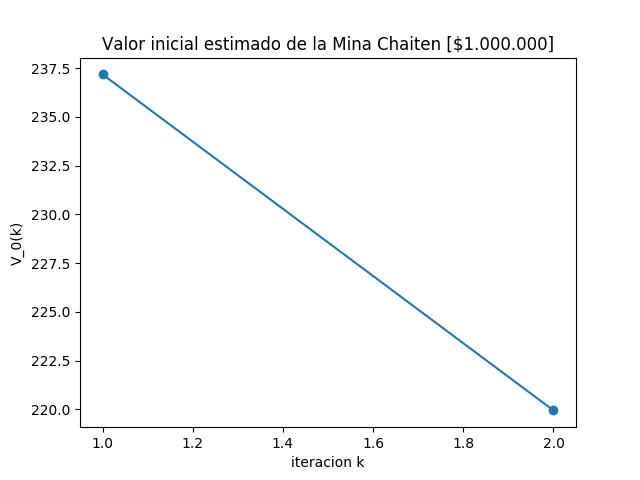
\includegraphics[width=\textwidth]{Graficos/Incrementos_filtrados/restringido/chaiten_inc_v_k.png}
     \caption{}
     \label{fig:ex2}
  \end{subfigure}

  \textbf{Incrementos sin filtrar (Libre)}
  
  \begin{subfigure}[b]{0.4\textwidth}
     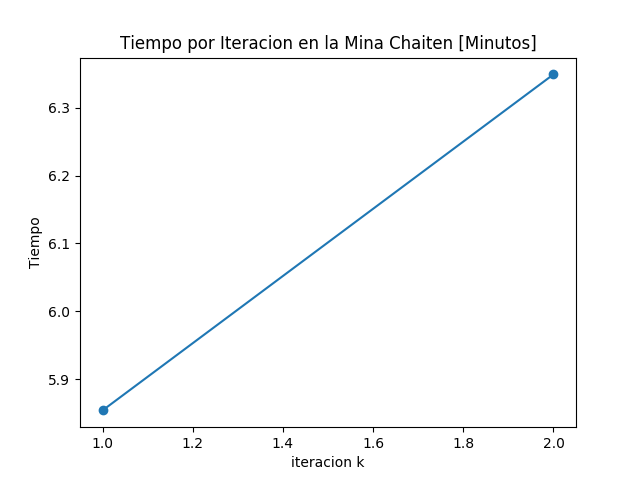
\includegraphics[width=\textwidth]{Graficos/sin_filtrar/libre/chaiten_inc_times.png}
     \caption{}
     \label{fig:ex1}
  \end{subfigure}
  \begin{subfigure}[b]{0.4\textwidth}
     \includegraphics[width=\textwidth]{Graficos/sin_filtrar/libre/chaiten_inc_v_k.png}
     \caption{}
     \label{fig:ex2}
  \end{subfigure}
\end{figure}

\begin{figure}
  \captionsetup[subfigure]{labelformat=empty}
  \centering
  \textbf{Incrementos sin filtrar (Restringido)}
  
  \begin{subfigure}[b]{0.4\textwidth}
     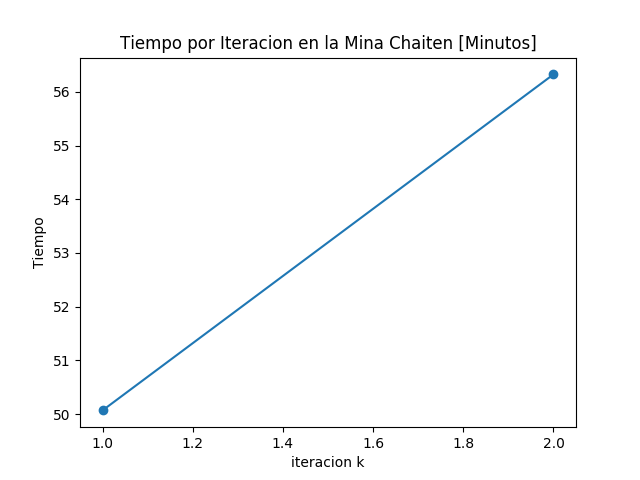
\includegraphics[width=\textwidth]{Graficos/sin_filtrar/restringido/chaiten_inc_times.png}
     \caption{}
     \label{fig:ex1}
  \end{subfigure}
  \begin{subfigure}[b]{0.4\textwidth}
     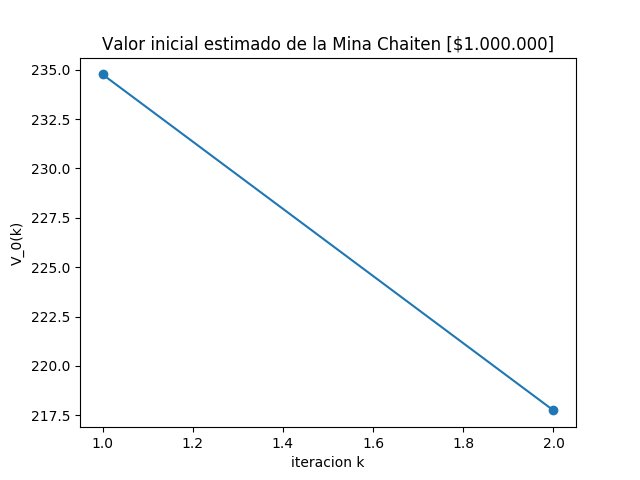
\includegraphics[width=\textwidth]{Graficos/sin_filtrar/restringido/chaiten_inc_v_k.png}
     \caption{}
     \label{fig:ex2}
  \end{subfigure}
\end{figure}

\subsubsection{Gráficos Kd}

\begin{figure}[H]
  \captionsetup[subfigure]{labelformat=empty}
  \centering
  
   \textbf{Incrementos filtrados (Libre)}
  
  \begin{subfigure}[b]{0.4\textwidth}
     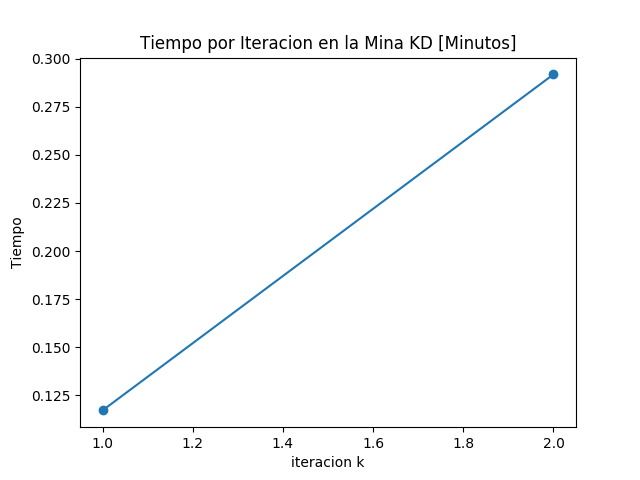
\includegraphics[width=\textwidth]{Graficos/Incrementos_filtrados/libre/kd_inc_times.png}
     \caption{}
     \label{asda}
  \end{subfigure}
  \begin{subfigure}[b]{0.4\textwidth}
     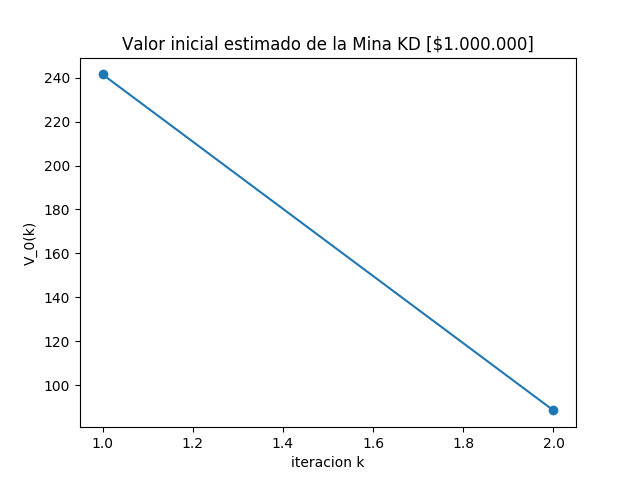
\includegraphics[width=\textwidth]{Graficos/Incrementos_filtrados/libre/kd_inc_v_k.png}
     \caption{}
     \label{fig:ex2}
  \end{subfigure}
  
  \textbf{Incrementos filtrados (Restringido)}
  
  \begin{subfigure}[b]{0.4\textwidth}
     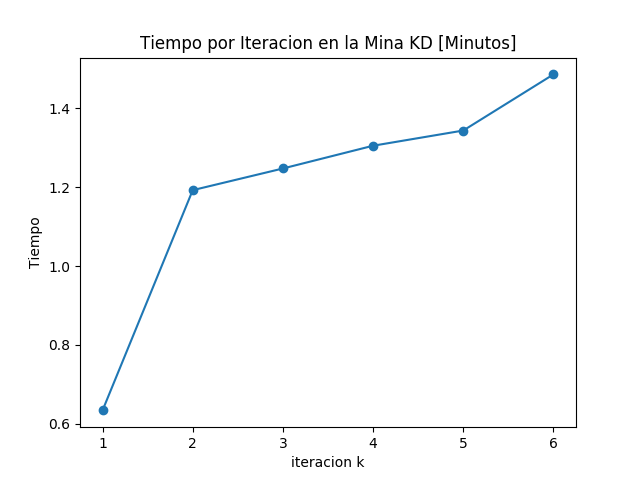
\includegraphics[width=\textwidth]{Graficos/Incrementos_filtrados/restringido/kd_inc_times.png}
     \caption{}
     \label{fig:ex1}
  \end{subfigure}
  \begin{subfigure}[b]{0.4\textwidth}
     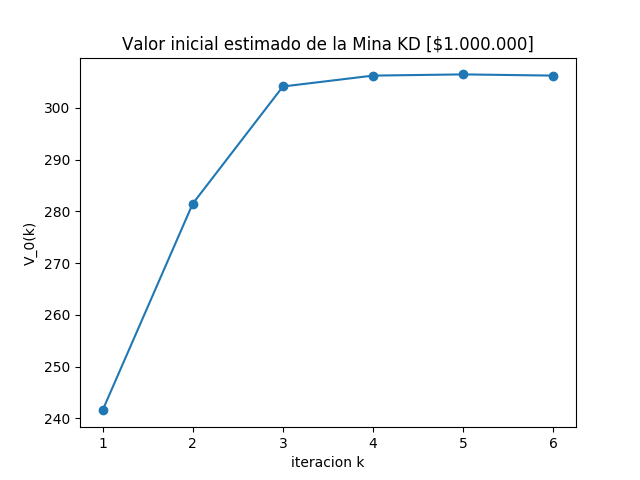
\includegraphics[width=\textwidth]{Graficos/Incrementos_filtrados/restringido/kd_inc_v_k.png}
     \caption{}
     \label{fig:ex2}
  \end{subfigure}
\end{figure}

\begin{figure}[H]
  \captionsetup[subfigure]{labelformat=empty}
  \centering
  \textbf{Incrementos Sin filtrar (Libres)}
  
  \begin{subfigure}[b]{0.4\textwidth}
     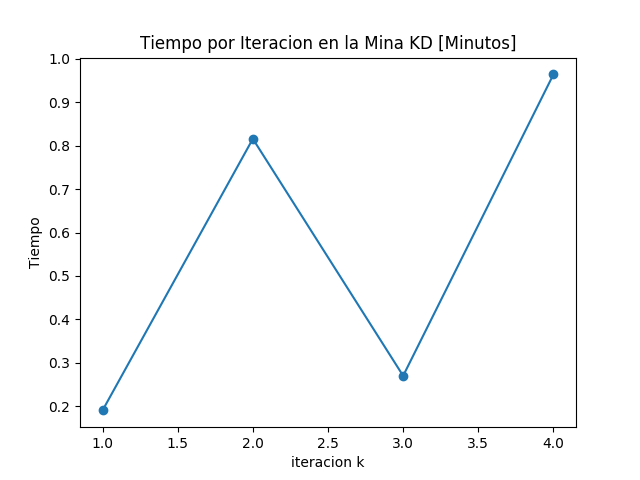
\includegraphics[width=\textwidth]{Graficos/sin_filtrar/libre/kd_inc_times.png}
     \caption{}
     \label{fig:ex1}
  \end{subfigure}
  \begin{subfigure}[b]{0.4\textwidth}
     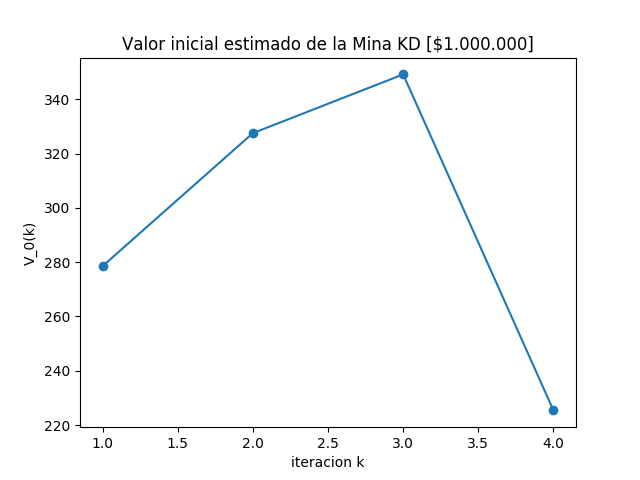
\includegraphics[width=\textwidth]{Graficos/sin_filtrar/libre/kd_inc_v_k.png}
     \caption{}
     \label{fig:ex2}
  \end{subfigure}

  \textbf{Incrementos Sin filtrar (restringidos)}
  
  \begin{subfigure}[b]{0.4\textwidth}
     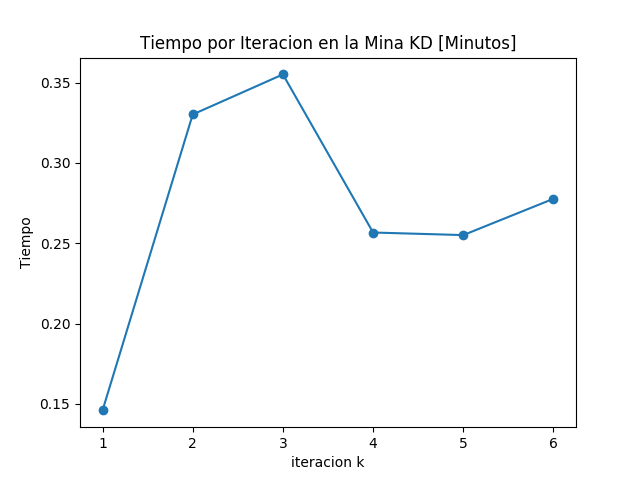
\includegraphics[width=\textwidth]{Graficos/sin_filtrar/restringido/kd_inc_times.png}
     \caption{}
     \label{fig:ex1}
  \end{subfigure}
  \begin{subfigure}[b]{0.4\textwidth}
     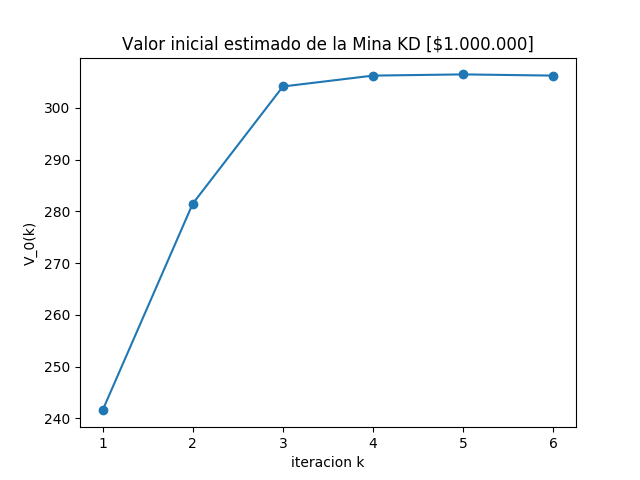
\includegraphics[width=\textwidth]{Graficos/Incrementos_filtrados/restringido/kd_inc_v_k.png}
     \caption{}
     \label{fig:ex2}
  \end{subfigure}
\end{figure}

\subsubsection{Gráficos Marvin}

\begin{figure}[H]
  \captionsetup[subfigure]{labelformat=empty}
  \centering
  
   \textbf{Incrementos filtrados (Libre)}
  
  \begin{subfigure}[b]{0.4\textwidth}
     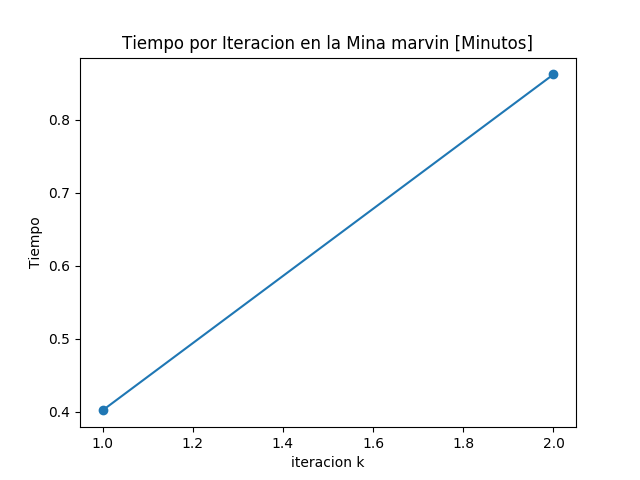
\includegraphics[width=\textwidth]{Graficos/Incrementos_filtrados/libre/marvinml_inc_times.png}
     \caption{}
     \label{asda}
  \end{subfigure}
  \begin{subfigure}[b]{0.4\textwidth}
     \includegraphics[width=\textwidth]{Graficos/Incrementos_filtrados/libre/marvinml_inc_v_k.png}
     \caption{}
     \label{fig:ex2}
  \end{subfigure}
\end{figure}

\begin{figure}[H]
  \captionsetup[subfigure]{labelformat=empty}
  \centering
  \textbf{Incrementos filtrados (Restringido)}
  
  \begin{subfigure}[b]{0.4\textwidth}
     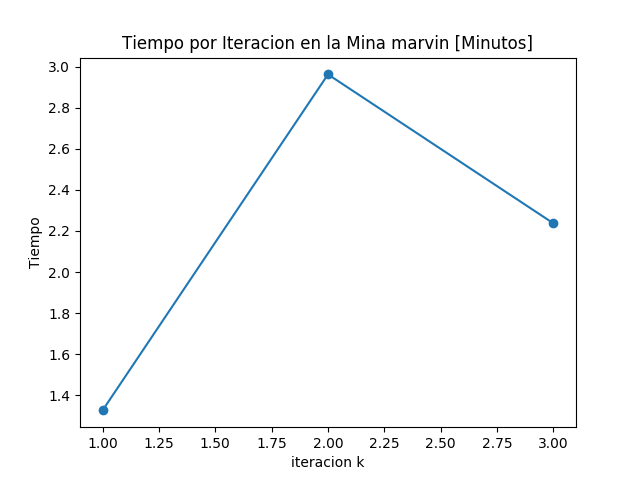
\includegraphics[width=\textwidth]{Graficos/Incrementos_filtrados/restringido/marvinml_inc_times.png}
     \caption{}
     \label{fig:ex1}
  \end{subfigure}
  \begin{subfigure}[b]{0.4\textwidth}
     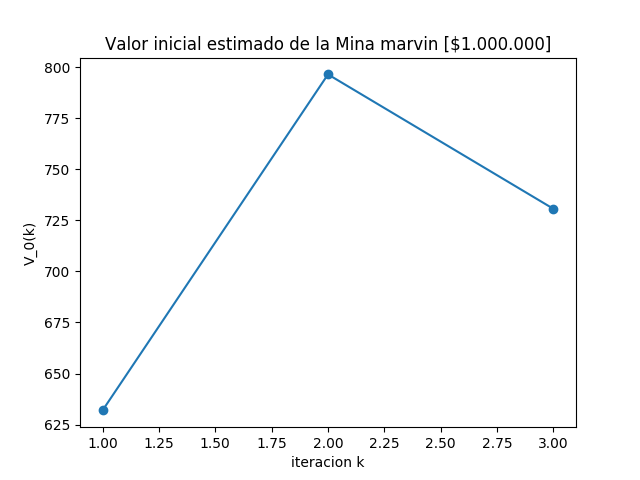
\includegraphics[width=\textwidth]{Graficos/Incrementos_filtrados/restringido/marvinml_inc_v_k.png}
     \caption{}
     \label{fig:ex2}
  \end{subfigure}
  
  \textbf{Incrementos sin filtrar (Libres)}
  
  \begin{subfigure}[b]{0.4\textwidth}
     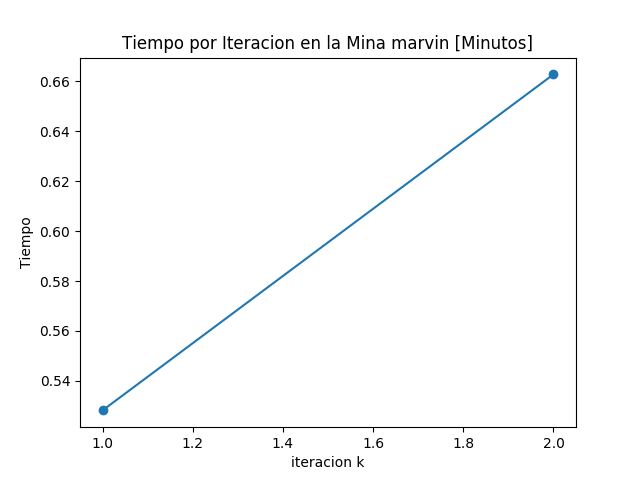
\includegraphics[width=\textwidth]{Graficos/sin_filtrar/libre/marvinml_inc_times.png}
     \caption{}
     \label{fig:ex1}
  \end{subfigure}
  \begin{subfigure}[b]{0.4\textwidth}
     \includegraphics[width=\textwidth]{Graficos/sin_filtrar/libre/marvinml_inc_v_k.png}
     \caption{}
     \label{fig:ex2}
  \end{subfigure}

  \textbf{Incrementos sin filtrar (Restringidos)}
  
  \begin{subfigure}[b]{0.4\textwidth}
     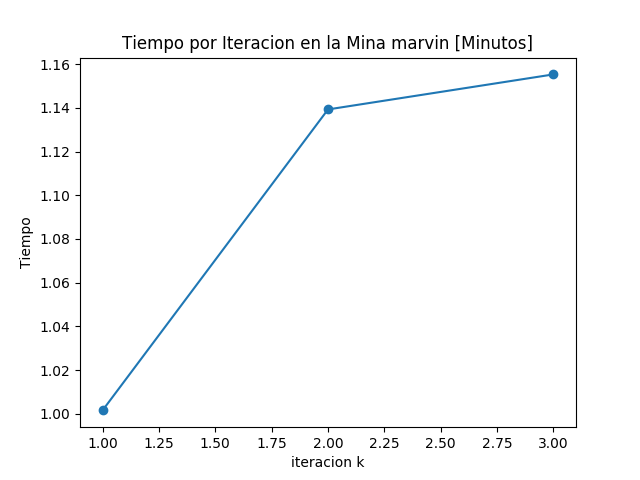
\includegraphics[width=\textwidth]{Graficos/sin_filtrar/restringido/marvinml_inc_times.png}
     \caption{}
     \label{fig:ex1}
  \end{subfigure}
  \begin{subfigure}[b]{0.4\textwidth}
     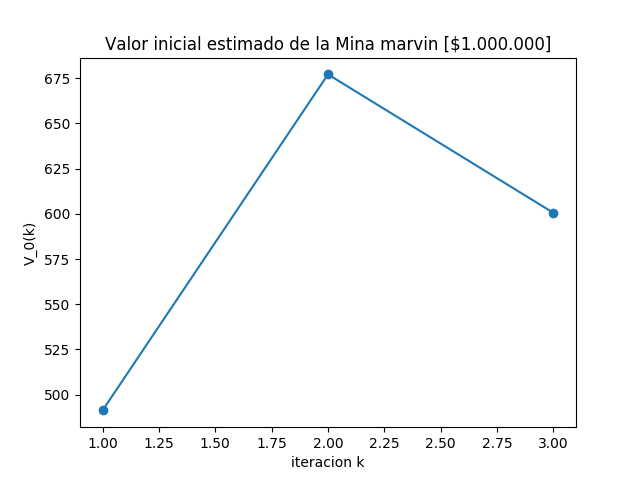
\includegraphics[width=\textwidth]{Graficos/sin_filtrar/restringido/marvinml_inc_v_k.png}
     \caption{}
     \label{fig:ex2}
  \end{subfigure}
\end{figure}

\newpage

\subsubsection{Gráficos Palomo}

\begin{figure}[H]
  \captionsetup[subfigure]{labelformat=empty}
  \centering
  \textbf{Incrementos filtrados (Libre)}
  
  \begin{subfigure}[b]{0.4\textwidth}
     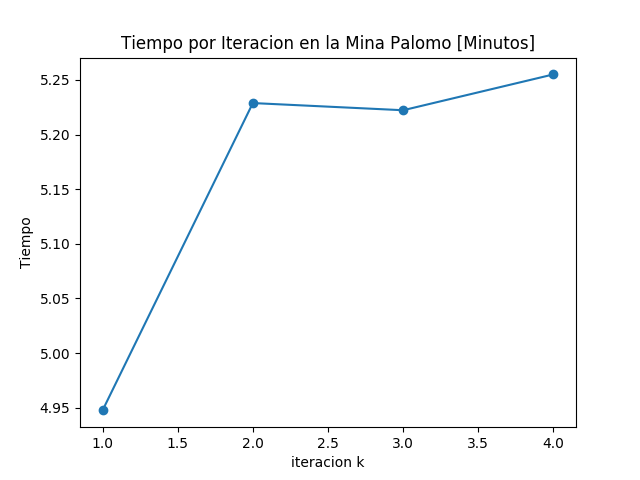
\includegraphics[width=\textwidth]{Graficos/Incrementos_filtrados/libre/palomo25_inc_times.png}
     \caption{}
     \label{fig:ex1}
  \end{subfigure}
  \begin{subfigure}[b]{0.4\textwidth}
     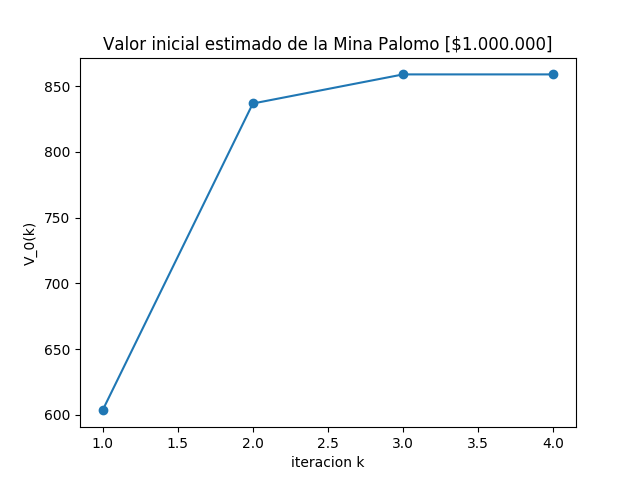
\includegraphics[width=\textwidth]{Graficos/Incrementos_filtrados/libre/palomo25_inc_v_k.png}
     \caption{}
     \label{fig:ex2}
  \end{subfigure}
  
  \textbf{Incrementos filtrados (Restringidos)}
  
  \begin{subfigure}[b]{0.4\textwidth}
     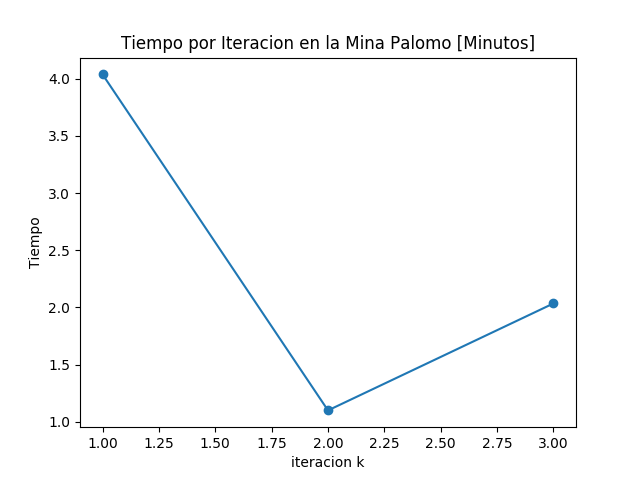
\includegraphics[width=\textwidth]{Graficos/Incrementos_filtrados/restringido/palomo25_inc_times.png}
     \caption{}
     \label{fig:ex1}
  \end{subfigure}
  \begin{subfigure}[b]{0.4\textwidth}
     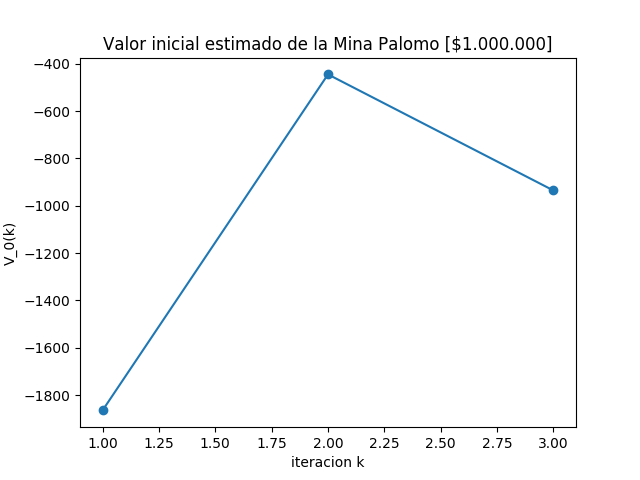
\includegraphics[width=\textwidth]{Graficos/Incrementos_filtrados/restringido/palomo25_inc_v_k.png}
     \caption{}
     \label{fig:ex2}
  \end{subfigure}

  \textbf{Incrementos sin filtrar (Libre)}
  
  \begin{subfigure}[b]{0.4\textwidth}
     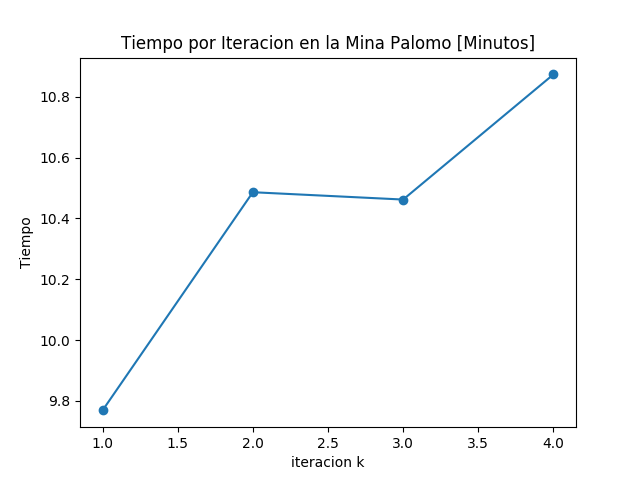
\includegraphics[width=\textwidth]{Graficos/sin_filtrar/libre/palomo25_inc_times.png}
     \caption{}
     \label{fig:ex1}
  \end{subfigure}
  \begin{subfigure}[b]{0.4\textwidth}
     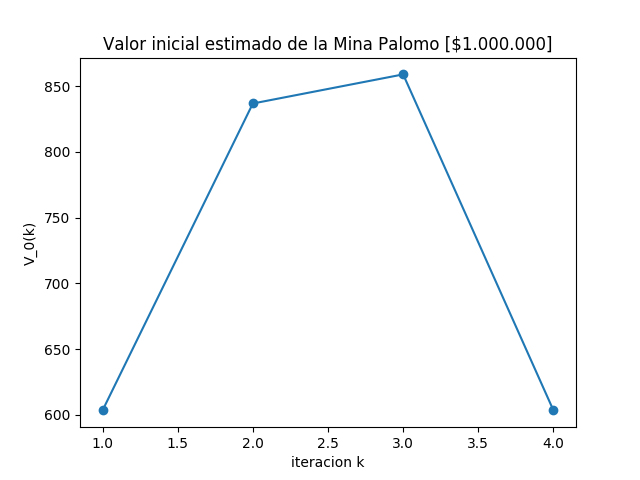
\includegraphics[width=\textwidth]{Graficos/sin_filtrar/libre/palomo25_inc_v_k.png} 
     \caption{}
     \label{fig:ex2}
  \end{subfigure}
\end{figure}

\newpage

\begin{figure}[H]
  \captionsetup[subfigure]{labelformat=empty}
  \centering
  \textbf{Incrementos sin filtrar (Restringidos)}
  
  \begin{subfigure}[b]{0.4\textwidth}
     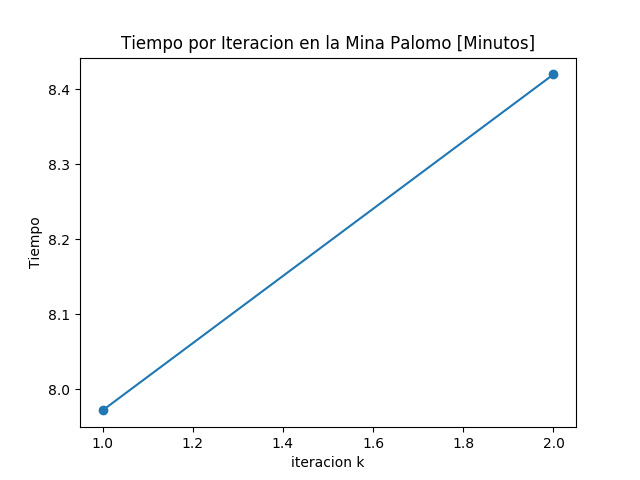
\includegraphics[width=\textwidth]{Graficos/sin_filtrar/restringido/palomo25_inc_times.png}
     \caption{}
     \label{fig:ex1}
  \end{subfigure}
  \begin{subfigure}[b]{0.4\textwidth}
     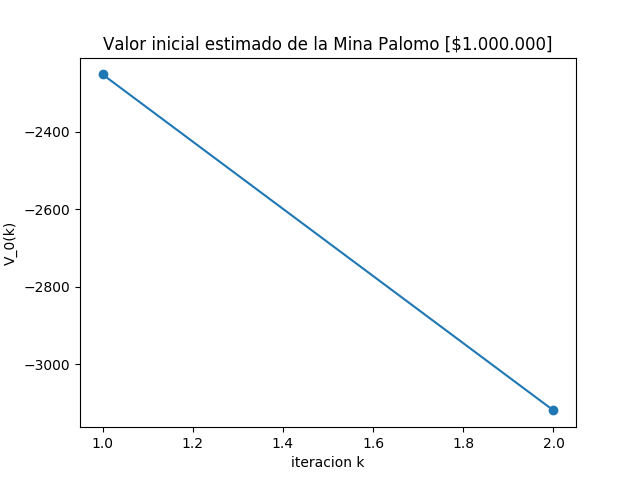
\includegraphics[width=\textwidth]{Graficos/sin_filtrar/restringido/palomo25_inc_v_k.png}
     \caption{}
     \label{fig:ex2}
  \end{subfigure}
\end{figure}

\subsection{Precedencias Ordenadas (Condición de Cauchy)}

\subsubsection{Chaitén}

\begin{figure}[H]
  \captionsetup[subfigure]{labelformat=empty}
  \centering
  \textbf{Incrementos Restringidos}
  
  \begin{subfigure}[b]{0.4\textwidth}
     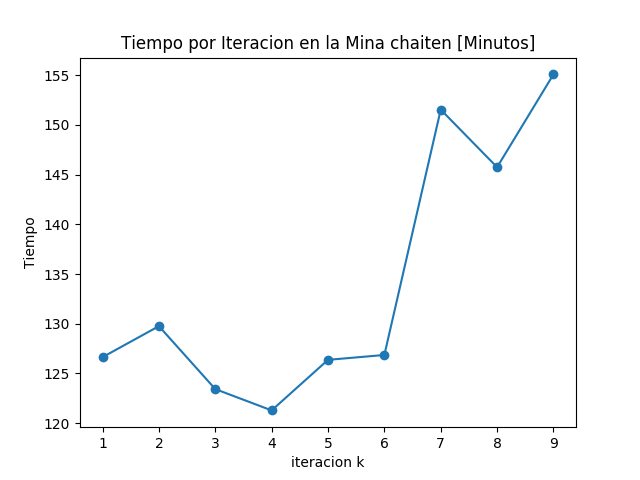
\includegraphics[width=\textwidth]{Graficos/FiltradosCauchyRestringidos/chaiten_inc_times..png}
     \caption{}
     \label{fig:ex1}
  \end{subfigure}
  \begin{subfigure}[b]{0.4\textwidth}
     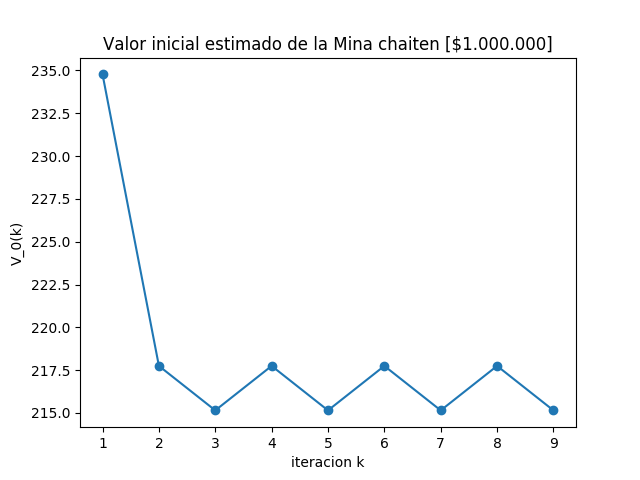
\includegraphics[width=\textwidth]{Graficos/FiltradosCauchyRestringidos/chaiten_inc_v_k..png}
     \caption{}
     \label{fig:ex2}
  \end{subfigure}
\end{figure}

\begin{figure}[H]
  \captionsetup[subfigure]{labelformat=empty}
  \centering
  \textbf{Incrementos Libres}
  
  \begin{subfigure}[b]{0.4\textwidth}
     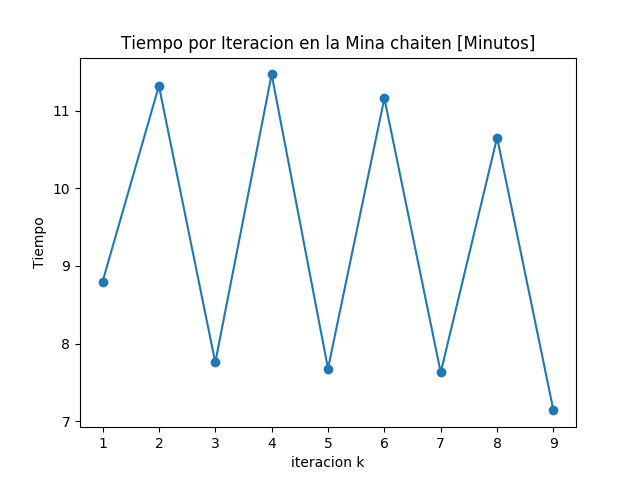
\includegraphics[width=\textwidth]{Graficos/FiltradosCauchyLibre/chaiten_inc_times..png}
     \caption{}
     \label{fig:ex1}
  \end{subfigure}
  \begin{subfigure}[b]{0.4\textwidth}
     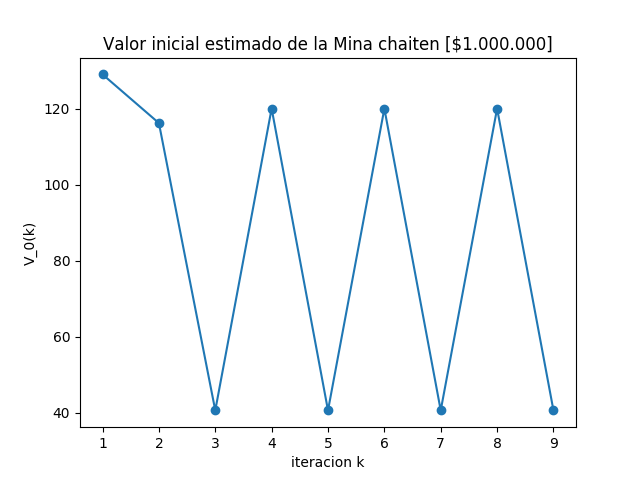
\includegraphics[width=\textwidth]{Graficos/FiltradosCauchyLibre/chaiten_inc_v_k..png}
     \caption{}
     \label{fig:ex2}
  \end{subfigure}
\end{figure}

\subsubsection{KD}

\begin{figure}[H]
  \captionsetup[subfigure]{labelformat=empty}
  \centering
  \textbf{Incrementos Restringidos}
  
  \begin{subfigure}[b]{0.4\textwidth}
     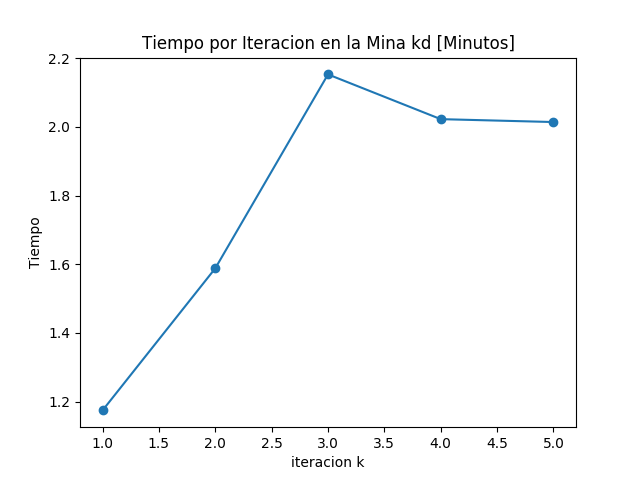
\includegraphics[width=\textwidth]{Graficos/FiltradosCauchyRestringidos/kd_inc_times..png}
     \caption{}
     \label{fig:ex1}
  \end{subfigure}
  \begin{subfigure}[b]{0.4\textwidth}
     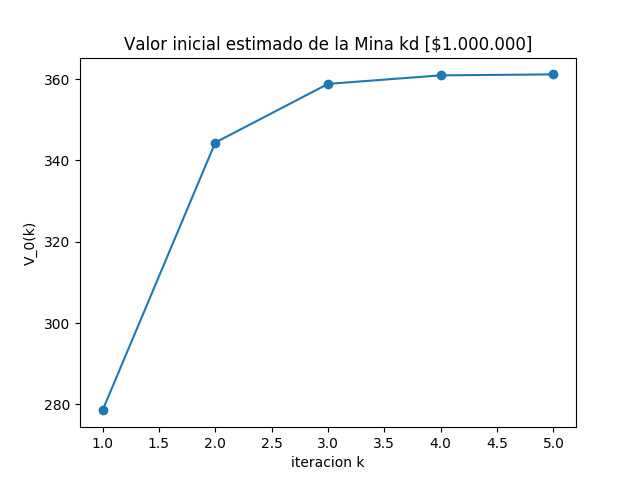
\includegraphics[width=\textwidth]{Graficos/FiltradosCauchyRestringidos/kd_inc_v_k..png}
     \caption{}
     \label{fig:ex2}
  \end{subfigure}
\end{figure}

\begin{figure}[H]
  \captionsetup[subfigure]{labelformat=empty}
  \centering
  \textbf{Incrementos Libres}
  
  \begin{subfigure}[b]{0.4\textwidth}
     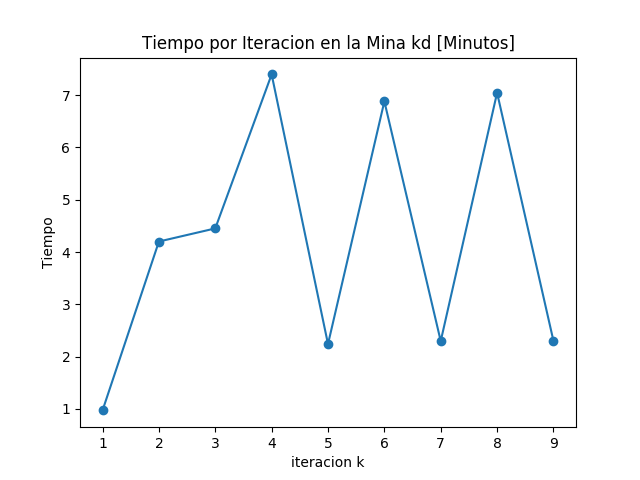
\includegraphics[width=\textwidth]{Graficos/FiltradosCauchyLibre/kd_inc_times..png}
     \caption{}
     \label{fig:ex1}
  \end{subfigure}
  \begin{subfigure}[b]{0.4\textwidth}
     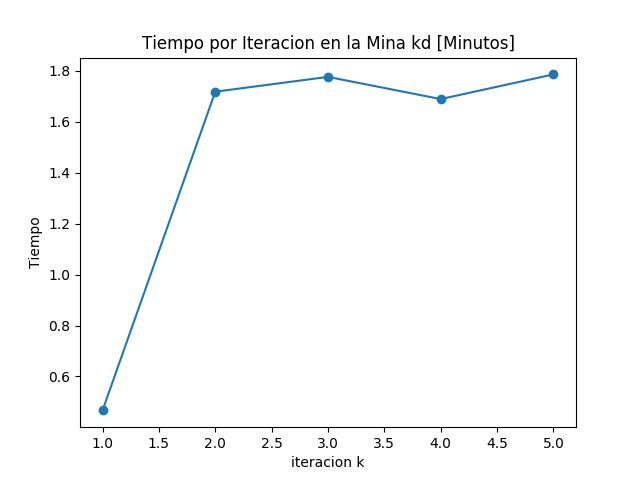
\includegraphics[width=\textwidth]{Graficos/Modelo2_Libre_Cauchy/kd_inc_times..png}
     \caption{}
     \label{fig:ex2}
  \end{subfigure}
\end{figure}

\subsubsection{Marvin}

\begin{figure}[H]
  \captionsetup[subfigure]{labelformat=empty}
  \centering
  \textbf{Incrementos Restringidos}
  
  \begin{subfigure}[b]{0.4\textwidth}
     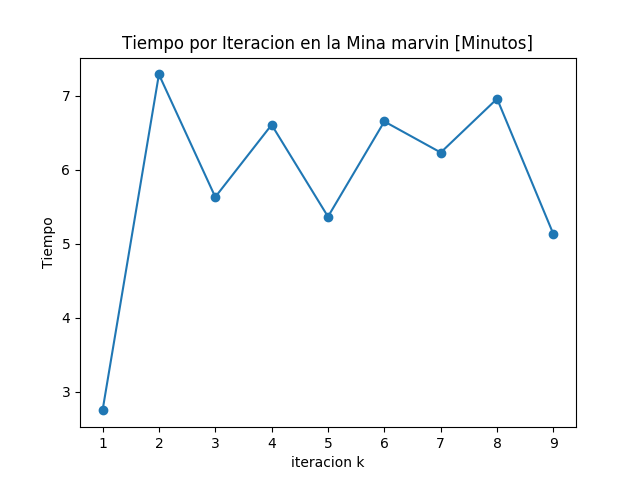
\includegraphics[width=\textwidth]{Graficos/FiltradosCauchyRestringidos/marvinml_inc_times..png}
     \caption{}
     \label{fig:ex1}
  \end{subfigure}
  \begin{subfigure}[b]{0.4\textwidth}
     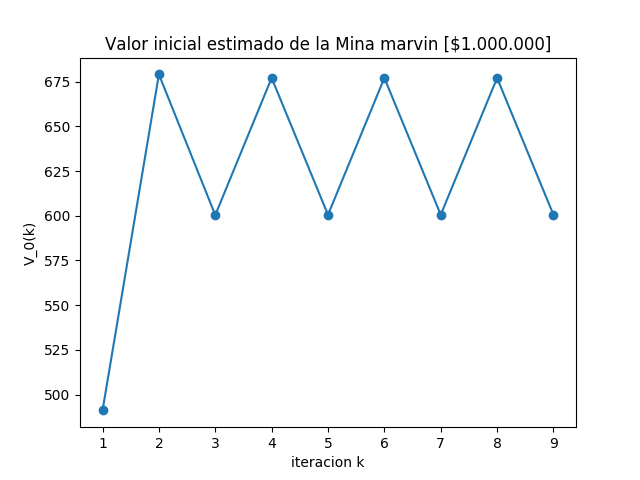
\includegraphics[width=\textwidth]{Graficos/FiltradosCauchyRestringidos/marvinml_inc_v_k..png}
     \caption{}
     \label{fig:ex2}
  \end{subfigure}
\end{figure}

\begin{figure}[H]
  \captionsetup[subfigure]{labelformat=empty}
  \centering
  \textbf{Incrementos Libres}
  
  \begin{subfigure}[b]{0.4\textwidth}
     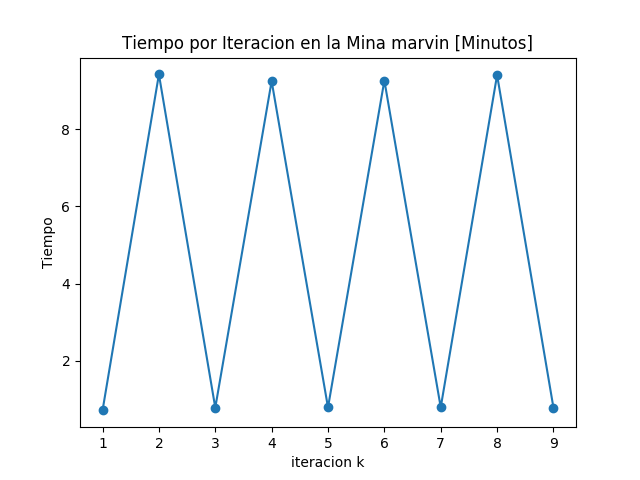
\includegraphics[width=\textwidth]{Graficos/FiltradosCauchyLibre/marvinml_inc_times..png}
     \caption{}
     \label{fig:ex1}
  \end{subfigure}
  \begin{subfigure}[b]{0.4\textwidth}
     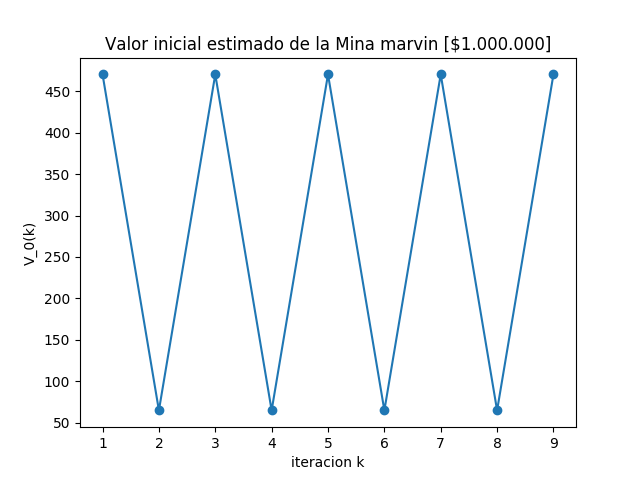
\includegraphics[width=\textwidth]{Graficos/FiltradosCauchyLibre/marvinml_inc_v_k..png}
     \caption{}
     \label{fig:ex2}
  \end{subfigure}
\end{figure}

\subsubsection{Palomo}

\section{Bibliografía}
\end{document}